\documentclass[11pt,a4paper]{article}

\usepackage{mynotes}

\usepackage{dcolumn}
\usepackage{multirow}
\usepackage{tikz}
\usetikzlibrary{calc,arrows,positioning,shapes,shapes.gates.logic.US,trees}
\usepackage{pdflscape}
\usepackage{longtable}

\title{An assessment of the biodiversity - ecosystem function relationship in southern African woodlands}
\author{John L. Godlee}
\date{}

\newcommand{\nplots}{1767}
\newcommand{\nplotspcoa}{1877}
\newcommand{\nstems}{93242}

\newcommand{\noutliers}{76}

\newcommand{\hullcover}{94.4}

\newcommand{\pcsdsd}{1}
\newcommand{\pcsded}{1.03}
\newcommand{\pcshdh}{1}
\newcommand{\pcshhh}{0.73}
\newcommand{\pcsdb}{-0.14}
\newcommand{\pcshb}{0.41}
\newcommand{\pcsdh}{0.42}
\newcommand{\pcsib}{0.77}
\newcommand{\pcsdi}{0.17}
\newcommand{\strucrsq}{0.7}
\newcommand{\strucbrsq}{0.69}
\newcommand{\struccrsq}{0.72}
\newcommand{\strucsib}{$\beta =$ NA$\pm$NA, p = NA}
\newcommand{\strucbsb}{$\beta =$ -0.25$\pm$0.064, p <0.01}
\newcommand{\strucbhb}{$\beta =$ 0.28$\pm$0.049, p <0.01}
\newcommand{\struccsb}{$\beta =$ 0.14$\pm$0.118, p = 0.24}

\newcommand{\rgmbd}{$\beta =$ 0.02$\pm$0.008, p = 0.06}
\newcommand{\rgsbd}{$\beta =$ 0.02$\pm$0.008, p = 0.05}
\newcommand{\rgid}{$\beta =$ 0.62$\pm$0.034, p <0.01}
\newcommand{\rghb}{$\beta =$ 0.33$\pm$0.042, p <0.01}
\newcommand{\fmrsq}{0.5}
\newcommand{\fmrmsea}{0.166}
\newcommand{\fmtli}{0.905}
\newcommand{\fmcfi}{0.924}
\newcommand{\pcfmmp}{1}
\newcommand{\pcfmmpc}{0.11}
\newcommand{\pcfmmt}{0.17}
\newcommand{\pcfmmtc}{0.57}
\newcommand{\pcfdds}{1}
\newcommand{\pcfdde}{0.72}
\newcommand{\pcfsss}{1}
\newcommand{\pcfsso}{0.31}
\newcommand{\pcfssc}{0.37}
\newcommand{\pcfhhh}{1}
\newcommand{\pcfhhd}{0.96}
\newcommand{\pcfmd}{0.21}
\newcommand{\pcfsd}{0.21}
\newcommand{\pcfdh}{0.3}
\newcommand{\pcfmi}{-0.01}
\newcommand{\pcfsi}{-0.01}
\newcommand{\pcfdi}{0.62}
\newcommand{\pcfsb}{0.03}
\newcommand{\pcfmb}{0.01}
\newcommand{\pcfdb}{0.07}
\newcommand{\pcfhb}{0.33}
\newcommand{\pcfib}{0.49}
\newcommand{\srsq}{46}

\newcommand{\ccib}{$\rho =$ 0.78, p <0.01}
\newcommand{\ccmb}{$\rho =$ 0.24, p <0.01}
\newcommand{\ccmcb}{$\rho =$ -0.09, p <0.01}
\newcommand{\ccob}{$\rho =$ 0.23, p <0.01}
\newcommand{\ccsb}{$\rho =$ -0.25, p <0.01}
\newcommand{\ccms}{$\rho =$ 0.39, p <0.01}
\newcommand{\ccme}{$\rho =$ 0.1, p <0.01}
\newcommand{\ccmh}{$\rho =$ 0.21, p <0.01}
\newcommand{\ccmi}{$\rho =$ 0.12, p <0.01}
\newcommand{\ccsi}{$\rho =$ 0.54, p <0.01}
\newcommand{\ccei}{$\rho =$ 0.47, p <0.01}
\newcommand{\cctb}{$\rho =$ -0.05, p <0.05}
\newcommand{\cctcb}{$\rho =$ -0.19, p <0.01}

\newcommand{\moderp}{$\beta =$ 0, t(1765) = 0.19, p = 0.85}
\newcommand{\moders}{$\beta =$ 0.02, t(1765) = 0.89, p = 0.38}

\newcommand{\subn}{80}
\newcommand{\subp}{359.4}


\begin{document}

\maketitle
\tableofcontents

\section{Introduction}

A large number of studies have shown relationships between biodiversity and ecosystem functionality \citep{Liang2016, Cardinale2009}. The strength and direction of these observed Biodiversity - Ecosystem Function Relationships (BEFRs) varies depending on the ecosystem being studied, the ecosystem function(s) of interest \citep{Hector2007}, and the inclusion of environmental covariates in statistical models \citep{Vila2005}, but there appears to be a generalisable positive correlation between biodiversity and ecosystem functionality \citep{Liang2016}. Over the past decade, many observational studies of the BEFR have been conducted, mostly in tropical and temperate forests, and grasslands \citep{Chen2011}. These studies support early findings from small scale experimental studies which began in earnest during the 1990s as concern grew over the global loss of biodiversity \citep{Tilman1994, Tilman2014}.

Ecosystem functions can be defined in broad terms as rate processes and properties of ecosystems which describe the degree of biotic activity within an ecosystem \citep{Jax2005}. This includes basic processes of primary production such as gross primary productivity and atmospheric nitrogen fixation, but can be extended to indirect aggregate measures of function such as resistance of productivity to disturbance, and even to static properties which themselves influence process, such as trophic complexity and total vegetative biomass. The frequently reported and intuitive relationship between biodiversity and ecosystem functionality invokes three main mechanisms which drive the relationship \citep{Tilman2014}: 1) niche complementarity, whereby communities with greater diversity fill a greater breadth of realised niche space and avoid competition due to differences in their traits, 2) selection effects, whereby communities with greater diversity are more likely to include a species which contributes highly to the measured ecosystem function, and 3) facilitation effects, whereby communities with greater diversity are more likely to include combinations of species which together increase the others functional contribution.

The relationship between biodiversity and ecosystem functionality has informed conservation policy which aims to maintain and strengthen biodiversity under the assumption that this strengthens ecosystem resilience to stressors such as anthropogenic climate change and ecosystem service use by humans \citep{Thompson2011}. It is probable however, that the strength and relative importance of the BEFR varies with ecosystem studied and environmental conditions, with many ecosystems remaining understudied in the BEFR literature.

The representation of dry tropical ecosystems in the BEFR literature is poor compared to other ecosystems. \citet{Clarke2017} conducted a meta-analysis of 182 published BEFR studies, finding that only 13\% were conducted in the tropics generally, with 42\% of those being conducted in the wet tropical forests of Costa Rica, which are unique in terms of species assemblage, being an oceanic island with many endemic species. In wet tropical forests, much of the observed effect of biodiversity on ecosystem function can be attributed to niche complementarity \citep{Wright2017, Poorter2015, Sande2017a}. In the dry tropics however, low precipitation, high seasonality of rainfall and temperature, and high levels of disturbance from fire and herbivory mean that niche complementarity and competition may not play as great a role in the relationship between biodiversity and ecosystem function. Instead, stress tolerance and the functional contribution of abundant species (selection effects) may be the predominant forces which influence ecosystem functionality \citep{Lasky2014, Tobner2016}. Similarly, more diverse species assemblages may lead to facilitation effects between certain species combinations in environments which are more hostile to growth \citep{Ratcliffe2017}.

Savannas and sparse woodlands are the dominant vegetation type across the southern African region, spanning >4 million km\textsuperscript{2} \citep{Ryan2016} (Figure \autoref{plot_loc}). The carbon stored in these woodlands is comparable to that found in the wet forests of the Congo basin and is of global importance to the carbon cycle \citep{Houghton2009, Mayaux2008}. Climatic conditions and biogeography vary across southern African woodlands, resulting in a diverse range of woodland tree species assemblages, which retain the common features of an open tree canopy and an understorey generally dominated by C4 grass species \citep{Frost1996}. Southern African woodlands are highly diverse, thought to harbour \textapprox{}8500 plant species of which there are >300 tree species \citep{Frost1996}. Southern African woodlands have been identified by previous studies as a priority for conservation efforts \citep{Brooks2006, Mittermeier2003}. Many conservation projects in the region currently aim to conserve biodiversity and woody biomass stocks simultaneously under the directive of the United Nations REDD+ programme or the similar Forest Carbon Partnership Facility (FCPF) \citep{Hinsley2015}. Despite these efforts however, human actions are driving rapid changes in biodiversity. Southern African woodlands are also relied heavily upon for their ecosystem service provision, which is itself affected by ecosystem functionality \citep{Schulze1994}. This has raised interest in how biodiversity influences ecosystem function in these ecosystems. Resource extraction by humans is directly influencing biodiversity via selective tree-felling for timber, charcoal making, non-timber forest products and through land use change to agriculture \citep{Aleman2016, Ryan2016}. Climate change is also indirectly affecting the biodiversity of southern African woodlands, altering temperature and precipitation, and affecting climate seasonality which heavily influences the degree of seasonal drought and thus woodland structure \citep{Scholes2004, Eldridge2012}. While rapid biodiversity change is being observed in southern African woodlands, research into the relationship between biodiversity and ecosystem functionality remains scarce.

A small number of academic studies in southern African woodlands have shown that above ground woody carbon/biomass stocks correlate positively with tree species richness \citep{McNicol2018, Shirima2015, Mutowo2012}, but the scientific impact of all these studies has been hampered by a restricted climatic and biogeographical range of study sites. Due to the highly variable environmental conditions within which southern African woodlands occur \citep{Frost1996}, and given the potential importance of environment and biogeography in defining the strength and form of a relationship between biodiversity and woody biomass, it is important to sample across these gradients to be able to infer a truly regional scale relationship between diversity and biomass. Studies conducted over small environmental gradients often find that at local scales, diversity shows a strong effect on ecosystem function, but at large scales diversity effects pale in significance compared to abiotic factors such as climate \citep{Pasari2013}. Small scale studies may therefore be over-estimating the effect of diversity.

In forests, climatic variation is known to affect both woody biomass \citep{Michaletz2014, Michaletz2018} and species diversity independently \citep{Spasojevic2014}, so it is important to account for climatic factors and understand how they interact with biomass and diversity to effectively model and correctly attribute the effects of biodiversity on biomass in analyses at large spatial scales in woodlands. \citet{Sankaran2005} used data from 854 African woodland field sites to show that mean annual precipitation (MAP) sets the upper limit for woody cover in savannas, which is positively correlated with biomass \citep{Chisholm2013, Prado-Junior2016}, while other factors such as herbivory, fire regime and soil properties also contribute at a local scale to reduce woody cover below this maximum. However, this study did not consider the role of species diversity in the complex interactions between environment and tree cover. 

Environmental conditions may indirectly moderate the observed relationship between biodiversity and ecosystem function \citep{Vila2005}. \citet{Condit2013} found that dry season intensity was the main determinant of tree species distribution and abundance evenness in Panamanian tropical forests. Dry season length may therefore indirectly affect ecosystem level productivity in forest ecosystems and thus woody biomass through selection effects, promoting the growth of a certain highly productive species only under specific environmental conditions. In European forests \citep{Ratcliffe2017} found a general trend towards stronger positive relationships between tree species richness and various ecosystem functions in more arid environments. They suggested variation in the balance between competitive and facilitative effects along the aridity gradient as the driver of this moderation relationship, an example of the Stress Gradient Hypothesis \citep{Dohn2013}. Water availability imposes a physiological limit on growth rate, which interacts with mortality due to stochastic processes such as fire and herbivory to limit maximum potential woody biomass \citep{Sankaran2005}. 

% Kunz et al. (2019) found that crown complementarity and crown plasticity increased with species richness. Trees growing in species rich neighbourhoods had enhanced AGB production in trunk and branches.

While southern African woodlands are species rich in the herbaceous understorey \citep{Murphy2016}, the tree layer is relatively species poor. \citet{Solbrig1996} however, writes that they remain structurally diverse in the tree layer, with trees occupying distinct layers of the canopy at different growth stages and between species. This structural diversity may be one mechanism through which diversity influences woody biomass. \citep{Kunz2019} found that crown complementarity and crown plasticity both increased with species richness in a seasonally dry subtropical forest. They also found that trees growing in species rich neighbourhoods exhibited enhanced biomass production. Tree species in southern African woodlands may differ in their occupation of different canopy layers allowing a more full canopy with a greater total foliage density, enhancing productivity and allowing greater standing woody biomass in a smaller area as a form of niche complementarity. This theory however, which has been supported by experiments and observational studies in temperate and wet tropical ecosystems \citep{Hardiman2011, Stark2012}, may not occur in savannas, which are structured by disturbance rather than competition. Instead, disturbance history may override the effects of species diversity on structural diversity nullifying the effects of species diversity on structural diversity.

\citep{Zhang2012} conducted a meta-analysis of 54 studies of the BEFR in forest ecosystems and found that greater tree species abundance evenness led to an increased effect size of species richness on productivity. They suggest this effect is caused by an increased heterogeneity of functional traits over space at small scales, leading to a more evenly filled environmental niche volume, which allows a greater number of species to maximise their productivity. We expect that this effect will occur in southern African woodlands as well. A decrease in species abundance evenness may be found as a result of increased disturbance, which prevents dominance by one species, or due to more extreme environmental conditions which preclude the growth of many species, instead favouring those few species who can effective tolerate sub-optimal conditions. It is important to therefore to consider not only species richness as a measure of diversity, but also the evenness of the distribution of trees among species when assessing the impact of diversity on ecosystem function.ecosystem function.

High levels of disturbance in the form of seasonal fires and herbivory from large mammals may moderate the strength of observable BEFRs in southern African woodlands \citep{Staver2009, Bond2005}. Fire disturbance in forests has been linked to abundance dependent mortality among smaller stems \citep{Roques2001}. A dominant and competitive species which tends to produce many small fast-growing stems is more likely to experience mortality during a fire as the higher surface area to volume ratio of the trunk increases the likelihood of combustion. These fast-growing bushy species exist in southern African woodlands and often proliferate when fire is deliberately excluded, leading to the growth of thicket vegetation which precludes the growth of high biomass tree species \citep{Higgins2007}. Additionally, the dominance of a single species is likely to decrease overall functioning by decreasing niche space utilisation \citep{Cardinale2002}.

In this study, we made the first known regional estimation of the Biodiversity-Ecosystem Function Relationship in southern African woodlands, using inventory plots which straddle multi-dimensional environmental and biogeographical gradients (Figure \autoref{plot_loc}, \autoref{temp_precip_hull}). We investigated the relationship between aboveground woody biomass and tree biodiversity. We compared the relative effects of tree species biodiversity with that of environmental factors known to affect ecosystem productivity and biomass accumulation: precipitation, temperature and soil fertility. We also investigated the potential moderation effects of environmental covariates on the relationship between tree species diversity and biomass. We incorporated vegetation type clusters based on major tree species compositional units into our analyses to understand how species composition as well as species biodiversity affected ecosystem functionality. Initially, we made four hypotheses: 

\subsection{Hypotheses}

\begin{enumerate}
	\item{Plots with a higher tree species diversity will maintain higher above-ground woody biomass stocks.}
	\item{More arid plots and plots with less fertile soil will show a stronger positive effect of tree species diversity on above-ground woody biomass.} 
	\item{There will be a positive effect of precipitation and soil fertility on AGB. Part of this positive effect will exist as a mediating effect through tree species diversity.}
	\item{Tree structural diversity of the woodland will interact with tree species diversity to provide an indirect path of influence between species diversity and woody biomass stocks.}
	\item{The observed effect of diversity on AGB will increase in strength as stem density increases owing to an increased importance of niche complementarity as competition increases.}
\end{enumerate}

To address these hypotheses we used Structural Equation Models with path analysis as a preferred method to simultaneously account for environmental factors and biotic factors, which may interact in their effect on ecosystem structure and therefore biomass.

\section{Methods}

\subsection{Study location}

The study used \nplots{} woodland monitoring plots from the larger SEOSAW network \citep{seosaw_web} located across 10 countries within southern Africa in so-called Miombo woodlands (\hyperref[plot_loc]{Figure~\ref*{plot_loc}}, \citealt{White1987}). The study region spans a precipitation gradient from \textapprox{}460 mm y\textsuperscript{-1} in southern Mozambique and southern Zimbabwe and \textapprox{}1700 mm y\textsuperscript{-1} in northern Zambia, Malawi and northern Mozambique. The study sites straddle the climate space of the region as a whole (\hyperref[temp_precip_hull]{Figure~\ref*{temp_precip_hull}}). The 2D convex hull of Mean Annual Precipitation (MAP) and Mean Annual Temperature (MAT) of the study sites covers \hullcover{}\% of the pixel-wise climate space of the Miombo woodland area as defined by \citet{White1987}, using WorldClim estimates of temperature and precipitation between the year 1970 and 2000 with a pixel size of 30 arc seconds (0.86 km\textsuperscript{2} at the equator) \citep{Fick2017}. 

\begin{figure}[H]
	\centering
	\subfloat[]{{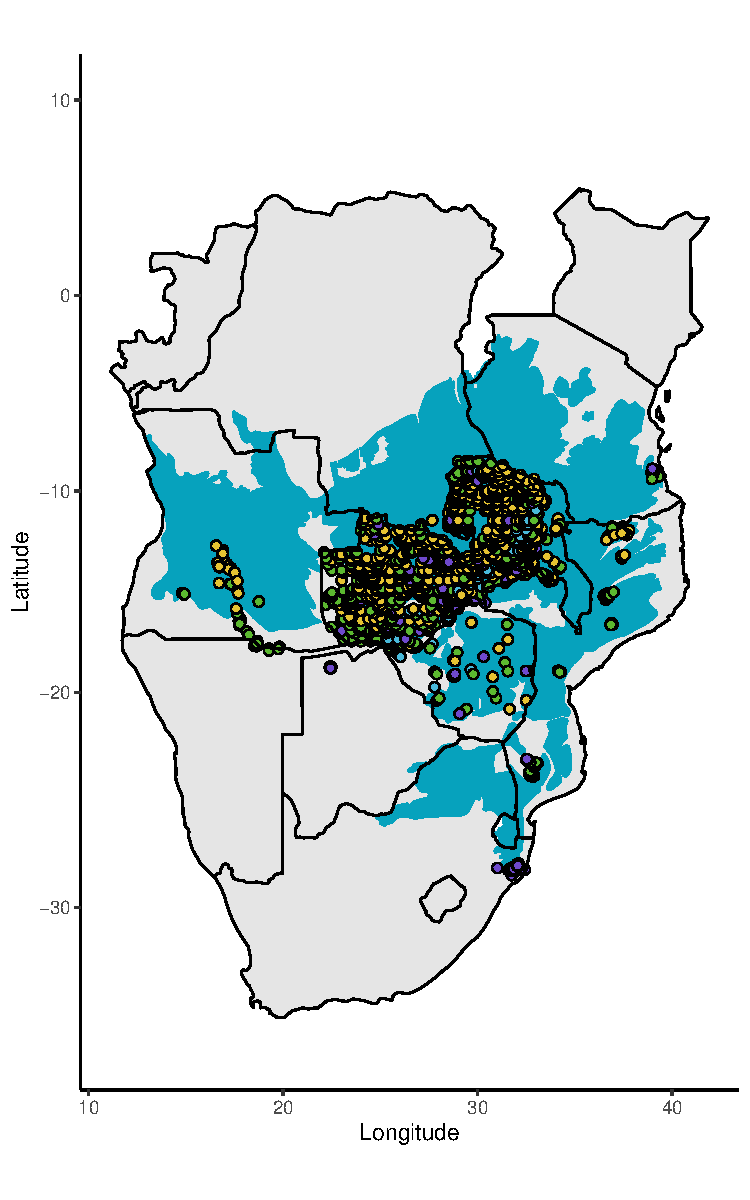
\includegraphics[width=0.3\textwidth]{plot_loc}}\label{plot_loc}}%
    \qquad
\subfloat[]{{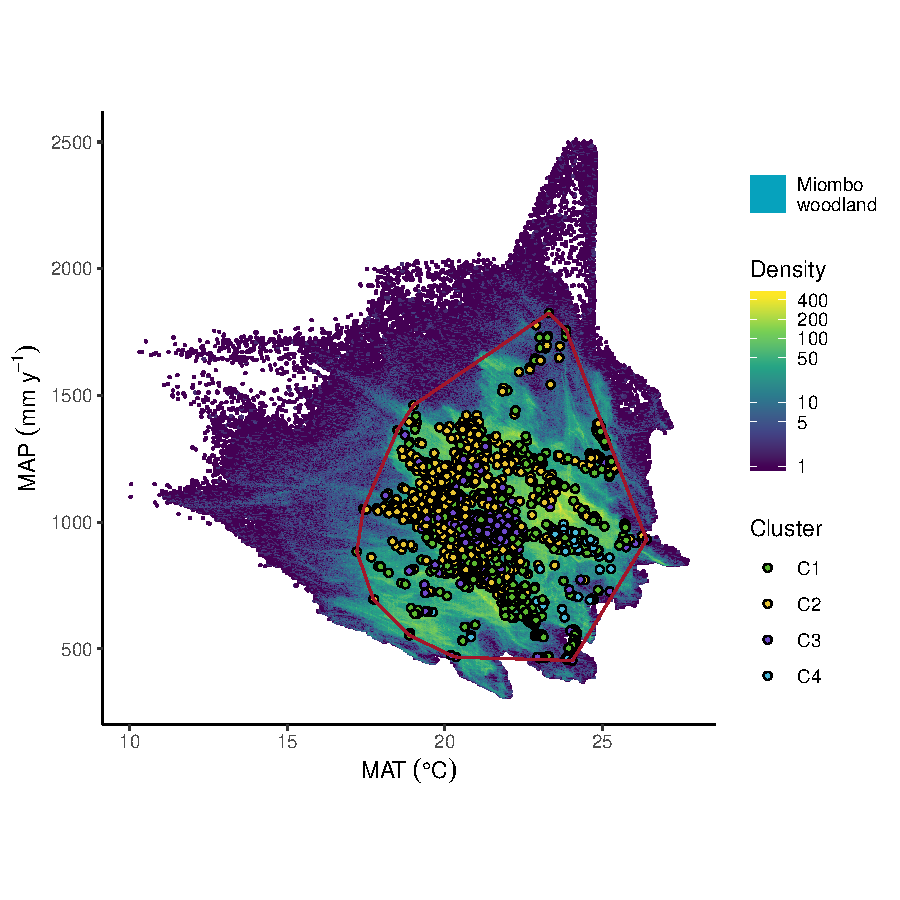
\includegraphics[width=0.4\textwidth]{temp_precip_hull}}\label{temp_precip_hull}}%
\caption{The locations of the \nplots{} plots used in this study, by geographic location (a) with respect to the distribution of Miombo woodland vegetation according to \citet{White1987}, and in climate space (b), showing the plot locations as points compared to the climate space of the whole region as estimated using the WorldClim dataset over the Miombo woodland vegetation extent \citep{Fick2017}. Note that the density colour scale is log-transformed.}
\end{figure}

Plots were chosen from a larger pool of 5395 plots based on the quality and completeness of data collection, and plot setup. Plot vegetation was identified under the broad term of ``savanna'', which includes ``woodland'', ``savanna woodland'', and ``tree savanna'', variously defined in other areas of the scientific literature \citep{Ratnam2011, Hill2010}. Plots with evidence of farming, human resource extraction or experimental treatments such as prescribed burning or herbivore exclusion were excluded from the initial pool. Only plots >0.1 hectares were used in analysis, as area based biomass estimation from small plots is highly influenced by rare large trees \citep{Stegen2011}, leading to inaccurate estimates. Only plots with a stem density >10 stems ha\textsuperscript{-1} were used, to ensure all plots were within woodland rather than ``grassy savanna'', which are considered a separate biome with very different species composition \citep{Parr2014} (\autoref{data_clean_flow}).

Many plots provided by the Zambian Forestry Commission were arranged in clusters of up to four 20x50 m plots, 20 metres apart. Plots within a cluster were aggregated before the plot dataset filtering described above and treated as a single plot in analyses.

After the initial plot data cleaning described above, we conducted an outlier removal procedure of plots with rare tree species composition. We used the \verb|outlier()| function from the \verb|dave| R package \citep{dave}, which uses a nearest neighbor criterion for each plot in species abundance ordination space and a threshold value for the minimum nearest neighbour distance to identify outliers. We set the threshold value to remove the top 5\% of plots with the largest nearest neighbour distances in multidimensional species composition space \citep{Otto2013}, removing \noutliers{} plots.

\subsection{Data collection}
 
We considered only trees and shrubs in our calculations of AGB, including woody species such as palms and cycads which are functionally tree-like but excluding lianas, which fill a different ecological niche \citep{Selaya2008}. Only stems >5 cm DBH (Diameter at Breast Height, 1.3 m) were included in analyses. Most plots in the dataset did not include data on stems <5 cm DBH, with these small stems comprising a very small proportion of the total AGB in a plot. 


All stems >5 cm DBH were measured within each plot resulting in a total of 160,076 stems with measurements. A tree may be comprised of multiple stems, but for this analysis each stem is treated as an individual. For each stem we measured species, DBH and tree height to the top of the highest branch material. Height was measured through a variety of means including laser rangefinders, manual clinometers and measuring sticks. When DBH could not be measured at 1.3 m due to trunk abnormalities, it was measured at the closest regular portion of the trunk to 1.3 m. The height of this measurement was recorded and used to estimate the DBH\textsubscript{e} at 1.3 m using a cubic polynomial regression, with parameters estimated using a test dataset from (Ryan, unpublished).

Woody AGB for each plot was calculated using \autoref{chave_agb}, taken from \citet{Chave2014}. Wood density estimates were taken from the global wood density database for each species where possible \citep{Chave2009, Zanne2009}. Wood density for species without species level estimates was estimated from the mean of their respective genus. 

\begin{equation}
	AGB = 0.0673 \times (\rho D^{2} H)^{0.976}
	\label{chave_agb}
\end{equation}

Where $\rho$ is the species level mean wood density, $D$ is the DBH at 1.3 m, and $H$ is the tree height.

Climatic data was collected from the ECMWF ERA5 dataset, generated using Copernicus Climate Change Service Information \citep{ERA5}. Values of Mean Annual Temperature (MAT) and Mean Annual Precipitation (MAP) were calculated from daily data between 2000 and 2018, then averaged across years to provide a single mean annual estimate per plot. Temperature and precipitation seasonality were both calculated as the coefficient of variation of daily MAT and MAP, respectively, across the 18 years of available data. Soil fertility data was extracted from the ISRIC gridded soil information data product at 250 m resolution, taking the grid cell value for each plot \citep{Hengl2017}. We extracted Cation Exchange Capacity (CEC), percentage soil organic carbon by volume (Org. C \%), and percentage soil sand content by volume (Sand \%). These data are a modelled product compiled from various remote sensed and directly measured data sources. 

% \todo{Fire return interval ($F_{ret}$) was calculated using the MODIS burned area product V6 (MCD46A1) \citep{}. Data was downloaded from January 2000 to December 2018. Mean fire return interval was calculated as:}
% 
% \begin{equation}
% 	\todo{F_{ret} = \frac{\sum_{i = 1}^{n} t_{i} - t_{i-1}}{n-1}}
% \end{equation}
% 
% \todo{Where $t_{i}$ is the date of fire $i$, and $n$ is the total number of fires in the time period.}

\subsection{Data analysis}
Estimated tree species richness was calculated for each plot using \verb|ChaoRichness()| from the \verb|iNEXT| package in R \citep{Hsieh2016}. This procedure uses Hill numbers to extrapolate a species rarefaction curve to its predicted asymptote and uses this value as its estimated species richness value. Extrapolated species richness was preferred over raw Hill numbers as they are more interpretable, representing actual species numbers. Extrapolated species richness accounts for variation in plot size (0.1-10 ha) and therefore sampling effort. Larger plots will tend to encompass more individuals, and therefore more species \citep{Dengler2009}.

To measure tree species abundance evenness, the Shannon Equitability index ($E_{H'}$) \citep{Smith1996} (\autoref{shannon_equit}) was calculated: 

\begin{equation}
	\begin{gathered}
		E_{H'} = \frac{H'_{e}}{\ln{S}} \\
	\end{gathered}
	\label{shannon_equit}
\end{equation}

Where $H'_{e}$ is an estimation of the Shannon diversity index of tree species by extrapolation of the observed Shannon diversity index ($H'$) to its asymptote via Hill numbers using the \verb|ChaoShannon()| function from the \verb|iNEXT| package in R \citep{Hsieh2016}, and $S$ is the extrapolated tree species richness in the plot. We calculated tree structural diversity for each plot by calculating the coefficient of variation of DBH and tree height. 

\subsubsection{Vegetation clusters}

Plots were assigned to vegetation type groups based on tree species composition. Groups were identified in \citet{Fayolle2018} using an Africa wide analysis of floristic units using plot data in savannas and woodlands with tree species diversity and relative abundance data. Groups were identified using unconstrained correspondence analysis and ordination. Plot data used in this study occurred in five vegetation type groups. See \autoref{clust_summ} for a description of each vegetation cluster and \autoref{clust_map} for the spatial distribution of plots from each of these clusters .

\begin{landscape}

% Table created by stargazer v.5.2.2 by Marek Hlavac, Harvard University. E-mail: hlavac at fas.harvard.edu
% Date and time: Thu, Dec 12, 2019 - 12:06:51
\begin{table}[!htbp] \centering 
  \caption{} 
  \label{clust_summ} 
\begin{tabular}{@{\extracolsep{5pt}} ccccccc} 
\\[-1.8ex]\hline 
\hline \\[-1.8ex] 
clust4 & c\_dom & c\_ind & n\_plots & n\_species\_raref & stems\_ha & agb\_ha \\ 
\hline \\[-1.8ex] 
1 & Julbernadia spp., Brachystegia spiciformis, Baikeaea plurijuga & Diplorhynchus condylocarpon, Burkea africana, Pseudolachnostylis maprouneifolia & 679 & 11(11.1) & 172(148) & 37.6(34.88) \\ 
2 & Julbernadia spp., Brachystegia spp., Isoberlinia angolensis & Julbernardia paniculata, Isoberlinia angolensis, Brachystegia longifolia & 746 & 18(17.5) & 216(170) & 49.1(43.34) \\ 
3 & Spirostachys africana, Senegalia spp., Euclea racemosa & Baikiaea plurijuga, Senegalia ataxacantha, Combretum collinum & 225 & 10(10) & 166(160) & 46.2(47.82) \\ 
4 & Colophospermum mopane & Colophospermum mopane, Combretum spp. & 99 & 7(8.2) & 190(155.7) & 41.5(36.93) \\ 
\hline \\[-1.8ex] 
\end{tabular} 
\end{table} 



\begin{figure}[H]
\centering
	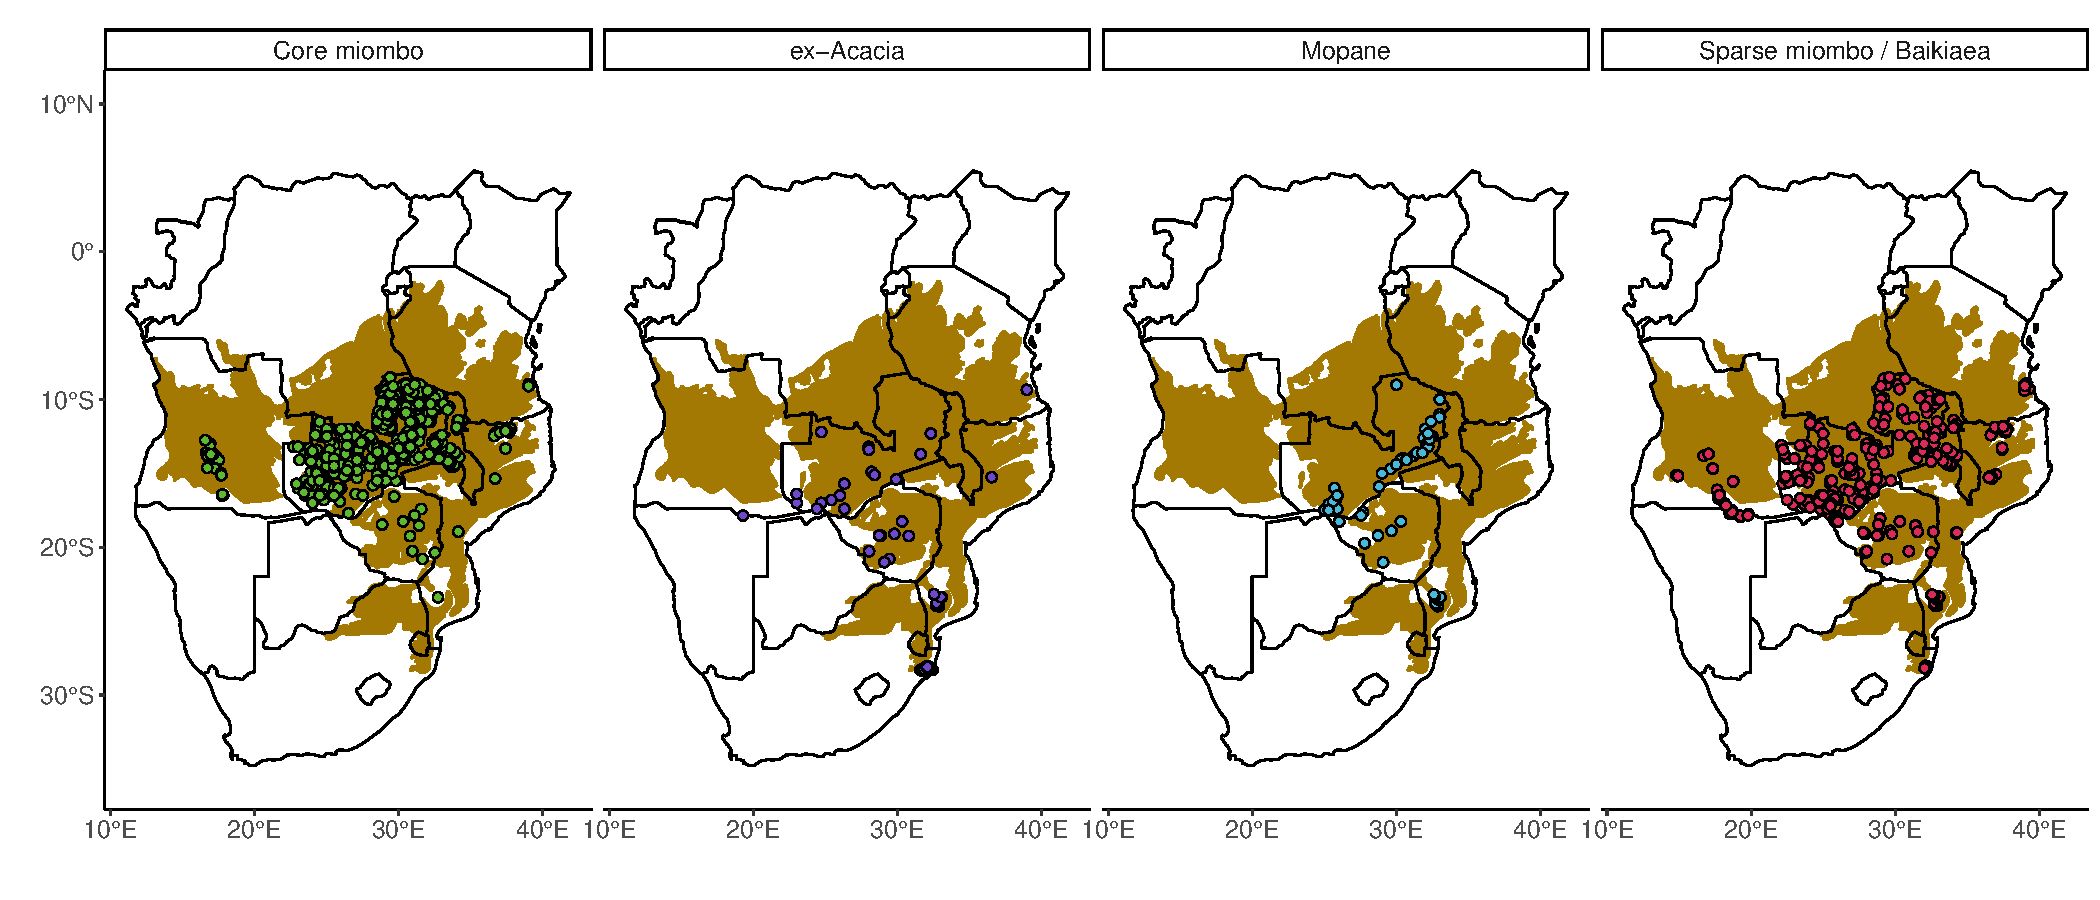
\includegraphics[width=0.8\textwidth]{clust_map}
	\caption{The spatial distribution of plots according to vegetation cluster within southern Africa.}
	\label{clust_map}
\end{figure}
\end{landscape}

\subsubsection{Structural Equation Modelling}

Structural Equation Models (SEM) investigated the determinants of AGB. All SEMs were constructed and analysed in the \verb|lavaan| package \citep{lavaan} in R version 3.6.0 \citep{R2019}. SEM was used because of its suitability for modelling complex causal interactions in ecological systems \citep{Lee2007}. A key aspect to our decision to use SEMs is that they can explicitly model and partition variance to indirect effects, which is impossible in multiple regression. Using SEMs also allowed us to describe theoretical latent constructs which have been suggested to act upon diversity and biomass/productivity in previous studies despite these factors not having single observable values in our dataset. For example, moisture availability is expected to affect AGB \citep{Saito2014, Campbell1996}, but moisture availability itself is determined by the interaction of multiple observable variables over the time scales relevant to tree lifetime growth: precipitation, the seasonality of that precipitation and temperature which affects the rate of evapotranspiration. Independently of total precipitation, precipitation seasonality determines whether water arrives uniformly over a given time period or as a few high volume floods, the latter leading to much water being lost before it can be used for plant growth. Structural equation modelling is also necessary to properly account for potential feedback mechanisms between aspects of climate and woody species diversity, which could otherwise increase the chances of Type I error and wrongly attributing inference due to covariance of explanatory variables, if testing for significant effects of biodiversity on AGB using conventional regression analyses \citep{Nachtigall2003}.

Prior to analysis, we specified a conceptual model with factors expected to affect AGB: moisture availability, soil fertility, tree species diversity, tree structural diversity and stem density (\autoref{con_mod}). 

\begin{figure}[H]
\centering
	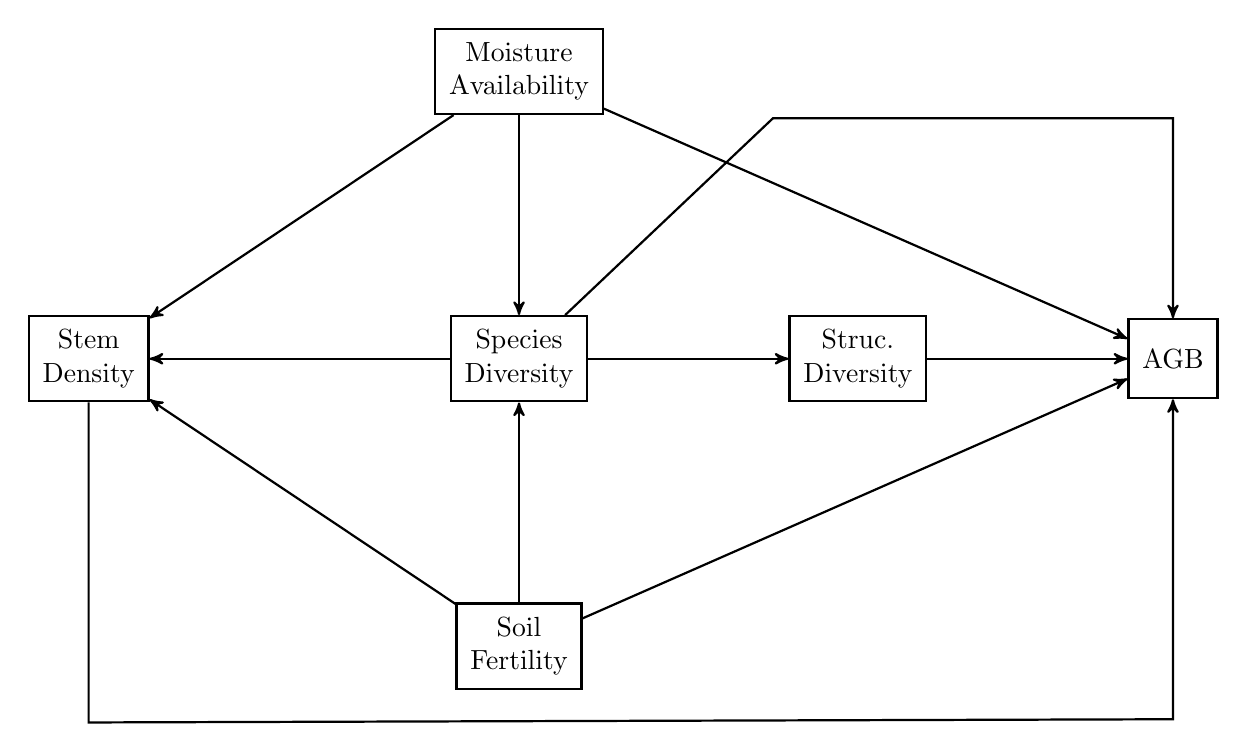
\begin{tikzpicture}[auto,scale=2, 
	observed/.style={rectangle,draw,thick,inner sep=5pt,minimum size=1cm, align=center},
	latent/.style={circle, draw, thick, inner sep=0pt, minimum size=2cm, align=center}, 
	path/.style={->, thick, >=stealth'},
	loading/.style={->, thick, dashed, >=stealth'}]

\tikzset{mystyle/.style={->,double=black}}
\node [observed] (m) {Moisture\\Availability};
\node [observed] (d) [below = 1in of m] {Species\\Diversity}; 
\node [observed] (s) [below = 1in of d] {Soil\\Fertility}; 
\node [observed] (h) [right = 1in of d] {Struc.\\Diversity}; 
\node [observed] (b) [right = 1in of h] {AGB}; 
\node [observed] (i) [left = 1.5in of d] {Stem\\Density};

\draw [path] (m) to node {} (d);
\draw [path] (s) to node[right] {} (d);
\draw [path] (d) to node[below] {} (h);
\draw [path] (h) to node {} (b);
\draw [path] (m) to node[above=0.1in, pos=0.5] {} (i);
\draw [path] (s) to node {} (i);
\draw [path] (d) to node {} (i);
\draw [path] (m) to node {} (b);
\draw [path] (s) to node[below=0.1in, pos=0.5] {} (b);

\coordinate[below= 1.6in of i] (ibleft); 
\coordinate[below= 1.6in of b] (ibright); 
\draw [path] (i) -- (ibleft) -- (ibright) -- (b);

\coordinate[above= 1in of b] (dbright);
\coordinate[left= 2in of dbright] (dbleft);
\draw [path] (d) -- (dbleft) -- (dbright) -- (b);
\end{tikzpicture}



	\caption{Conceptual Directed Acyclic Graph (DAG) showing the theoretical relationships between environmental factors, tree species diversity, tree structural diversity, tree stem density, and AGB. Hypothesised paths of causation are depicted as arrows from predictor to response.}
	\label{con_mod}
\end{figure}

Observed variables were standardised to Z-scores prior to analysis. Standardization put each latent variable on the same scale, with a mean of zero and a standard deviation of one. Standardization allows path regression coefficients to be easily compared between paths in the same model to assess their relative effect strength, and eliminates confusion in model interpretation arising from the observed variables being on different scales \citep{Beaujean2014}. Standardization also controls for variables with different orders of magnitude which could otherwise prevent adequate model estimation from the covariance matrix in \verb|lavaan|. To ensure that observed variables within a latent variable had consistent directions of influence, some observed variables were reversed by multiplying by -1. For example, soil fertility is expected to decrease as soil sand content increases, so soil percentage sand content was reversed for model fitting. Precipitation seasonality, temperature seasonality, and mean temperature were also reversed in this way to account for the direction of their effect on moisture availability.

The factor loadings of the observed variable assumed to contribute most to each latent variable were set to 1 as per convention, with other observed variables being allowed to vary \citep{Beaujean2014}. While it is recommended by some to set exact factor loadings in the SEM from the regression coefficients of multiple regressions \citep{lavaan}, because some latent variables were regressed against both structural diversity and AGB, exact factor loadings from simple multiple regressions could not be used. We therefore allowed factor loadings to be estimated by the SEM itself. We tested the robustness of our assumptions with a chi-squared test of all possible combinations of observed variable factor loadings set to 1, finding no significant difference between model specifications. Full Information Max-Likelihood (FIML) was used in each model to estimate the values of missing data in each latent variable \citep{Cham2017}.

First, we assessed the interacting factors of structural diversity and species diversity in determining AGB. We constructed a simple mediation model which allowed species diversity to influence AGB both directly and indirectly via structural diversity. To explore variation in the model among woodland vegetation types, we fit the model both at the regional scale and for each vegetation cluster separately. We compared unstandardised path coefficients among these vegetation cluster scale models to understand the effect that vegetation type has on the relationship between tree species diversity, structural diversity, stem density and AGB. Path coefficients show the effect of a path with other paths of inference held constant. Model fit was evaluated using the Comparative Fit Index (CFI), the Tucker Lewis Index (TLI), the Root Mean Squared Error (RMSEA) and the R\textsuperscript{2} coefficient of determination for AGB. 

To explore the hypothesis that complementarity effects increase in strength as stem density increases, we repeatedly sub-sampled the available plot dataset to create 900 datasets of similar size with varying median stem density. We used each of these datasets to fit the model including only tree species and structural diversity latent variables to predict AGB. We then examined how the unstandardised path coefficients for each path in the SEM varied according to the median stem density of subsampled dataset.

Second, we incorporated environmental covariates into our model to understand the relative effects of moisture availability and soil fertility on AGB both directly and indirectly via species diversity and stem density. We compared standardised path coefficients between paths in the model to understand the relative contribution of each path to explain variance in AGB.

We fitted separate moderation models to investigate whether there was an interaction effect whereby the strength of the relationship between species diversity and AGB was influenced by moisture availability and soil fertility. The \verb|lavaan| R package does not natively support moderation of latent variables in its model specification. Instead we manually calculated interaction variables for both soil fertility and moisture availability from the product of predicted values of these latent variables in a Confirmatory Factor Analysis (CFA). Interaction variables were the products: tree species diversity $\times$ moisture availability, and tree species diversity $\times$ soil fertility. These interaction terms were included as explanatory terms in multiple regressions alongside the latent variable of species diversity to predict AGB. Regression coefficients and model fit were analysed to determine the presence and form of interaction effects.

\section{Results}

\begin{figure}[H]
\centering
	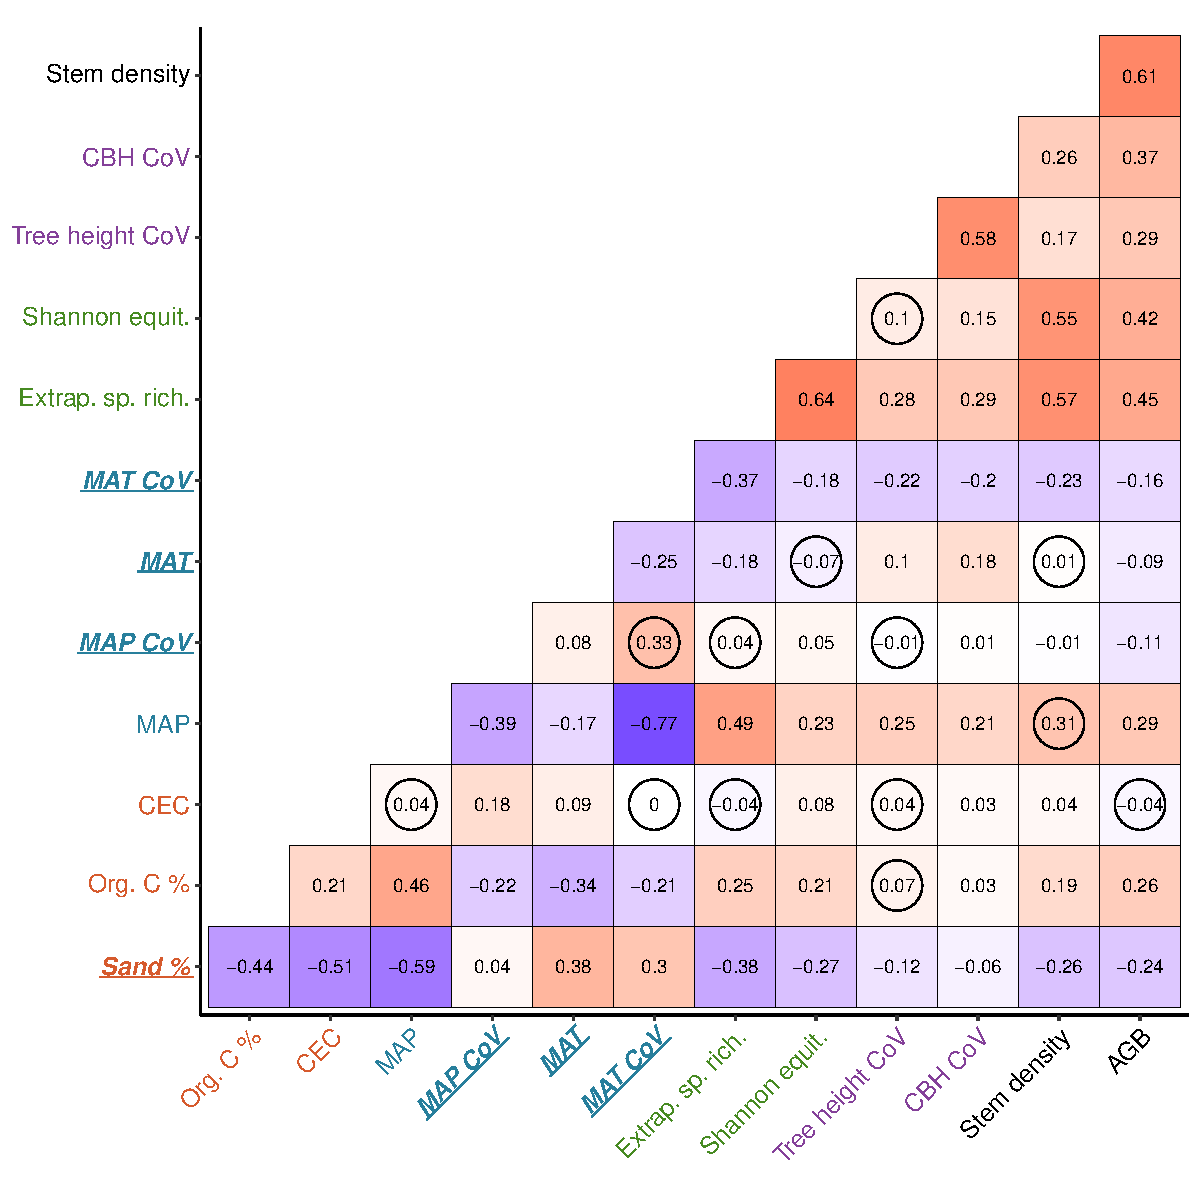
\includegraphics[width=0.6\textwidth]{corr_mat}
	\caption{Correlogram of standardised observed variables used in the SEMs, with Pearson correlation coefficients ($\rho$) coloured according to sign ($+$ve red, $-$ve blue) and shaded by strength of correlation. Variables in bold and underlined on the axis labels were later reversed for SEMs to maintain positive correlations for all observed variables within each latent variable. Correlation coefficients marked by a circle indicate that the 95\% confidence interval of this correlation overlapped zero. Colours of variable names group them into latent variables used in the SEMs: red = Soil fertility, blue = Moisture availability, green = tree species diversity, purple = tree structural diversity. See \autoref{corr_ci_tab} for a full assessment of correlation fit statistics.}
	\label{corr_mat}
\end{figure}

Pairwise correlations between all observed variables used in the Structural Equation Models (SEMs) showed that all tree species diversity and structural diversity variables had moderate positive correlations with AGB. Stem density had the strongest correlation with AGB of all variables (\ccib{}). Environmental variables had weaker correlations with AGB than diversity variables, with all environmental variables having significant correlations with AGB, except CEC.

The direction of these correlations was used as a test of our assumptions of the direction of influence of of latent variables later used in the SEMs. As expected, there was a positive correlation between MAP and AGB (\ccmb{}), and a negative correlation between the seasonality of precipitation and AGB (\ccmcb{}. MAT and the seasonality of temperature negatively correlated with AGB (MAT: \cctb{}; MAT seasonality: \cctcb{}). As expected, there was a negative correlation between soil sand content and AGB (\ccsb{}), and a positive correlation between soil organic Carbon and AGB (\ccob{}).

MAP had positive correlations with tree species richness (\ccms{}), abundance evenness (\ccme{}), tree height diversity (\ccmh{}) and a positive but not significant correlation with tree stem density. MAT had non significant correlations with tree species and structural diversity variables. Tree species diversity variables had clear positive correlations with stem density (Species richness: \ccsi{}; Shannon equitability: \ccei{}). 

\subsection{Structural and species diversity models}

In an SEM describing the effect of tree species diversity on AGB via the mediating effects of stand structural diversity and stem density (\autoref{struc_mod}), species diversity had a positive effect on AGB, both directly and indirectly via stem density and structural diversity (\autoref{struc_mod}, \autoref{struc_model_slopes}). Tree species diversity had a strong positive effect on stem density. Model fit was good with high factor loadings for all observed variables, all path coefficients were significant (p <0.01) (\autoref{struc_model_fit_clust_stats}). The R-squared of AGB was \strucrsq{}. The strongest effect of tree species diversity on AGB was via stem density (\strucsib{})


\begin{figure}[H]
\centering
	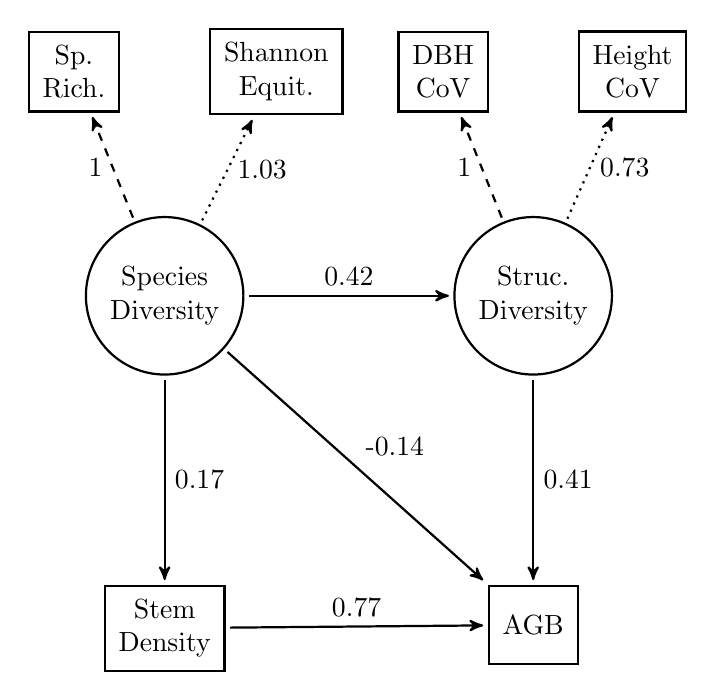
\begin{tikzpicture}[auto,scale=2, 
	observed/.style={rectangle,draw,thick,inner sep=5pt, outer sep=2pt, minimum size=1cm, align=center},
	latent/.style={circle, draw, thick, inner sep=0pt, outer sep=2pt, minimum size=2cm, align=center}, 
	path/.style={->, thick, >=stealth'},
	loading/.style={->, thick, dotted, >=stealth'},
	loadingset/.style={->, thick, dashed, >=stealth'}]

\tikzset{mystyle/.style={->,double=black}}
\node [latent] (d) {Species\\Diversity}; 
\node [latent] (h) [right = 1in of d] {Struc.\\Diversity}; 
\node [observed] (b) [below = 1in of h] {AGB}; 
\node [observed] (i) [below = 1in of d] {Stem\\Density};

\coordinate[above= 0.7in of d] (domid);
\coordinate[above= 0.7in of h] (homid);
\node [observed] (ds) [left = 0.2in of domid] {Sp.\\Rich.};
\node [observed] (de) [right = 0.2in of domid] {Shannon\\Equit.};
\node [observed] (hd) [left = 0.2in of homid] {DBH\\CoV};
\node [observed] (hh) [right = 0.2in of homid] {Height\\CoV};


\draw [loadingset] (d) to node[left, pos=0.5] {\pcsdsd{}} (ds);
\draw [loading] (d) to node[right, pos=0.5] {\pcsded{}} (de);
\draw [loadingset] (h) to node[left, pos=0.5]  {\pcshdh{}} (hd);
\draw [loading] (h) to node[right, pos=0.5] {\pcshhh{}} (hh);

\draw [path] (d) to node {\pcsdh{}} (h);
\draw [path] (h) to node {\pcshb{}} (b);
\draw [path] (d) to node {\pcsdi{}} (i);
\draw [path] (i) to node {\pcsib{}} (b);
\draw [path] (d) to node {\pcsdb{}} (b);

\end{tikzpicture}


	\caption{Path diagram with regression coefficients for the tree diversity SEM, including plots from all five vegetation clusters. Latent variables are shown as circles while observed variables are shown as rectangles. Path coefficients are solid arrows pointing from predictor to response. The observed variables which inform the unmeasured latent variables are connected by dotted arrows, observed variables with loading set to one are connected by dashed arrows. Measurement errors of exogenous variables are omitted for clarity.}
	\label{struc_mod}
\end{figure}

\begin{figure}[H]
\centering
	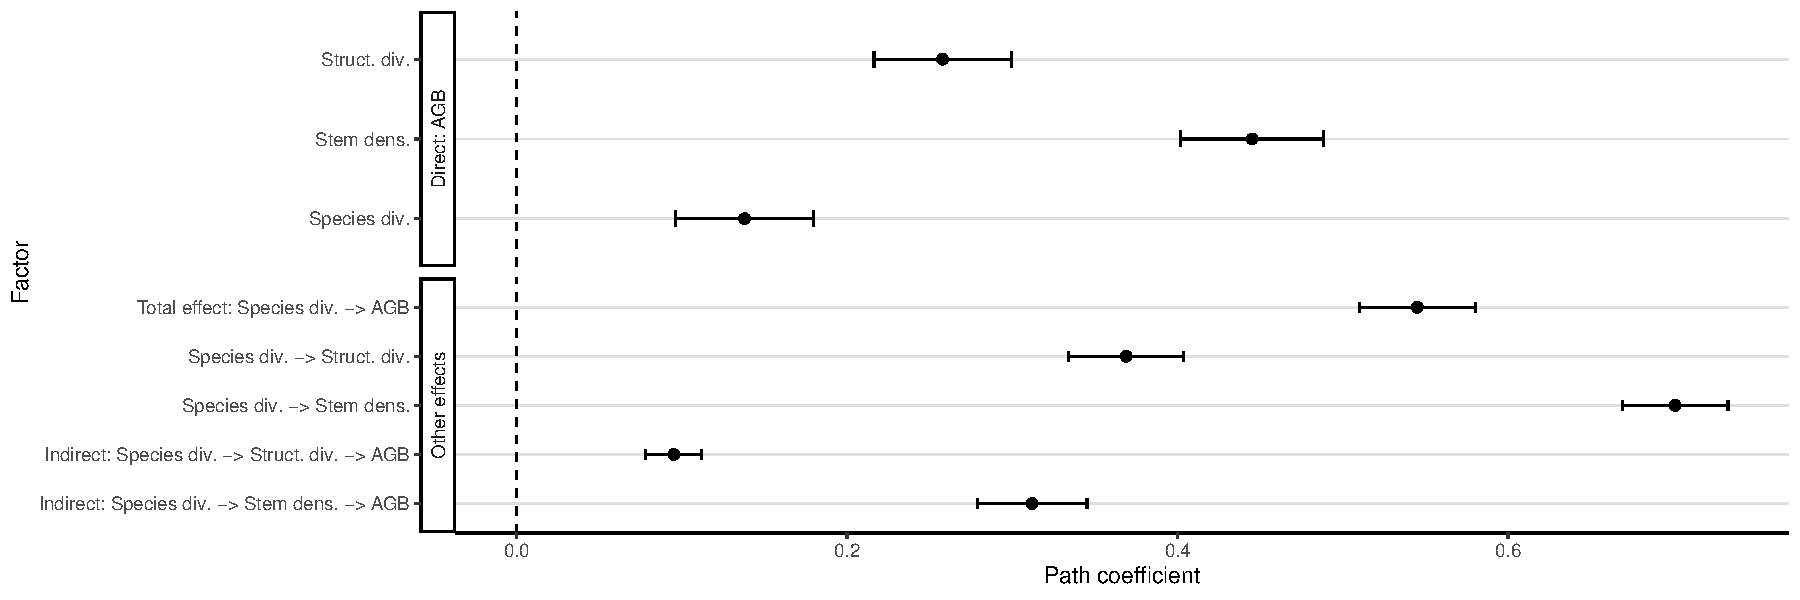
\includegraphics[width=\textwidth]{struc_model_slopes}
	\caption{Standardised path coefficients for the effects of tree diversity on AGB, mediated by the effect of stand structural diversity. Due to all observed variables being standardised and centred, path coefficients are expressed in terms of standard deviations on the latent variable response scale $\pm$1 standard error. Path coefficients where the standard error does not overlap zero are considered significant effects.}
	\label{struc_model_slopes}
\end{figure}

\subsection{Variation among vegetation clusters in structural and species diversity effects}

When the tree species and structural diversity model (\autoref{struc_mod}) was refitted separately using data from each of the 4 vegetation clusters the strengths of unstandardised path coefficients varied but relationships between tree diversity and AGB remained generally similar with the same sign and significant overlap between the 95\% confidence intervals of path coefficients. All models exhibited adequate goodness-of-fit (\autoref{struc_model_fit_clust_stats}), though wide confidence intervals around the unstandardised path coefficients, particularly for Clusters 3 and 4 indicate an issue with model prediction due to low sample size for these clusters. $\chi^{2}$ statistics were high for some vegetation clusters, but this appears to be highly correlated with sample size in our data \citep{}.

Cluster 2, which contained vegetation dominated by \textit{Julbernadia paniculata} showed no significant effect of tree species diversity on AGB (\strucbsb{}), in contrast to the other vegetation clusters, and had a significantly smaller positive effect of structural diversity on AGB (\strucbhb{}) (\autoref{struc_model_slopes_all}).

The strongest total effect of tree species diversity on AGB was in Cluster 3 (\struccsb{}), which was species rich but highly variable in species diversity compared to other vegetation clusters (\autoref{clust_summ}). The greatest effect of structural diversity on AGB was found in Clusters 3 and 4. The R-squared of AGB was highest in cluster 3 (R\textsuperscript{2} = \struccrsq{}) and lowest in cluster 2 (R\textsuperscript{2} = \strucbrsq{}).

\begin{figure}[H]
\centering
	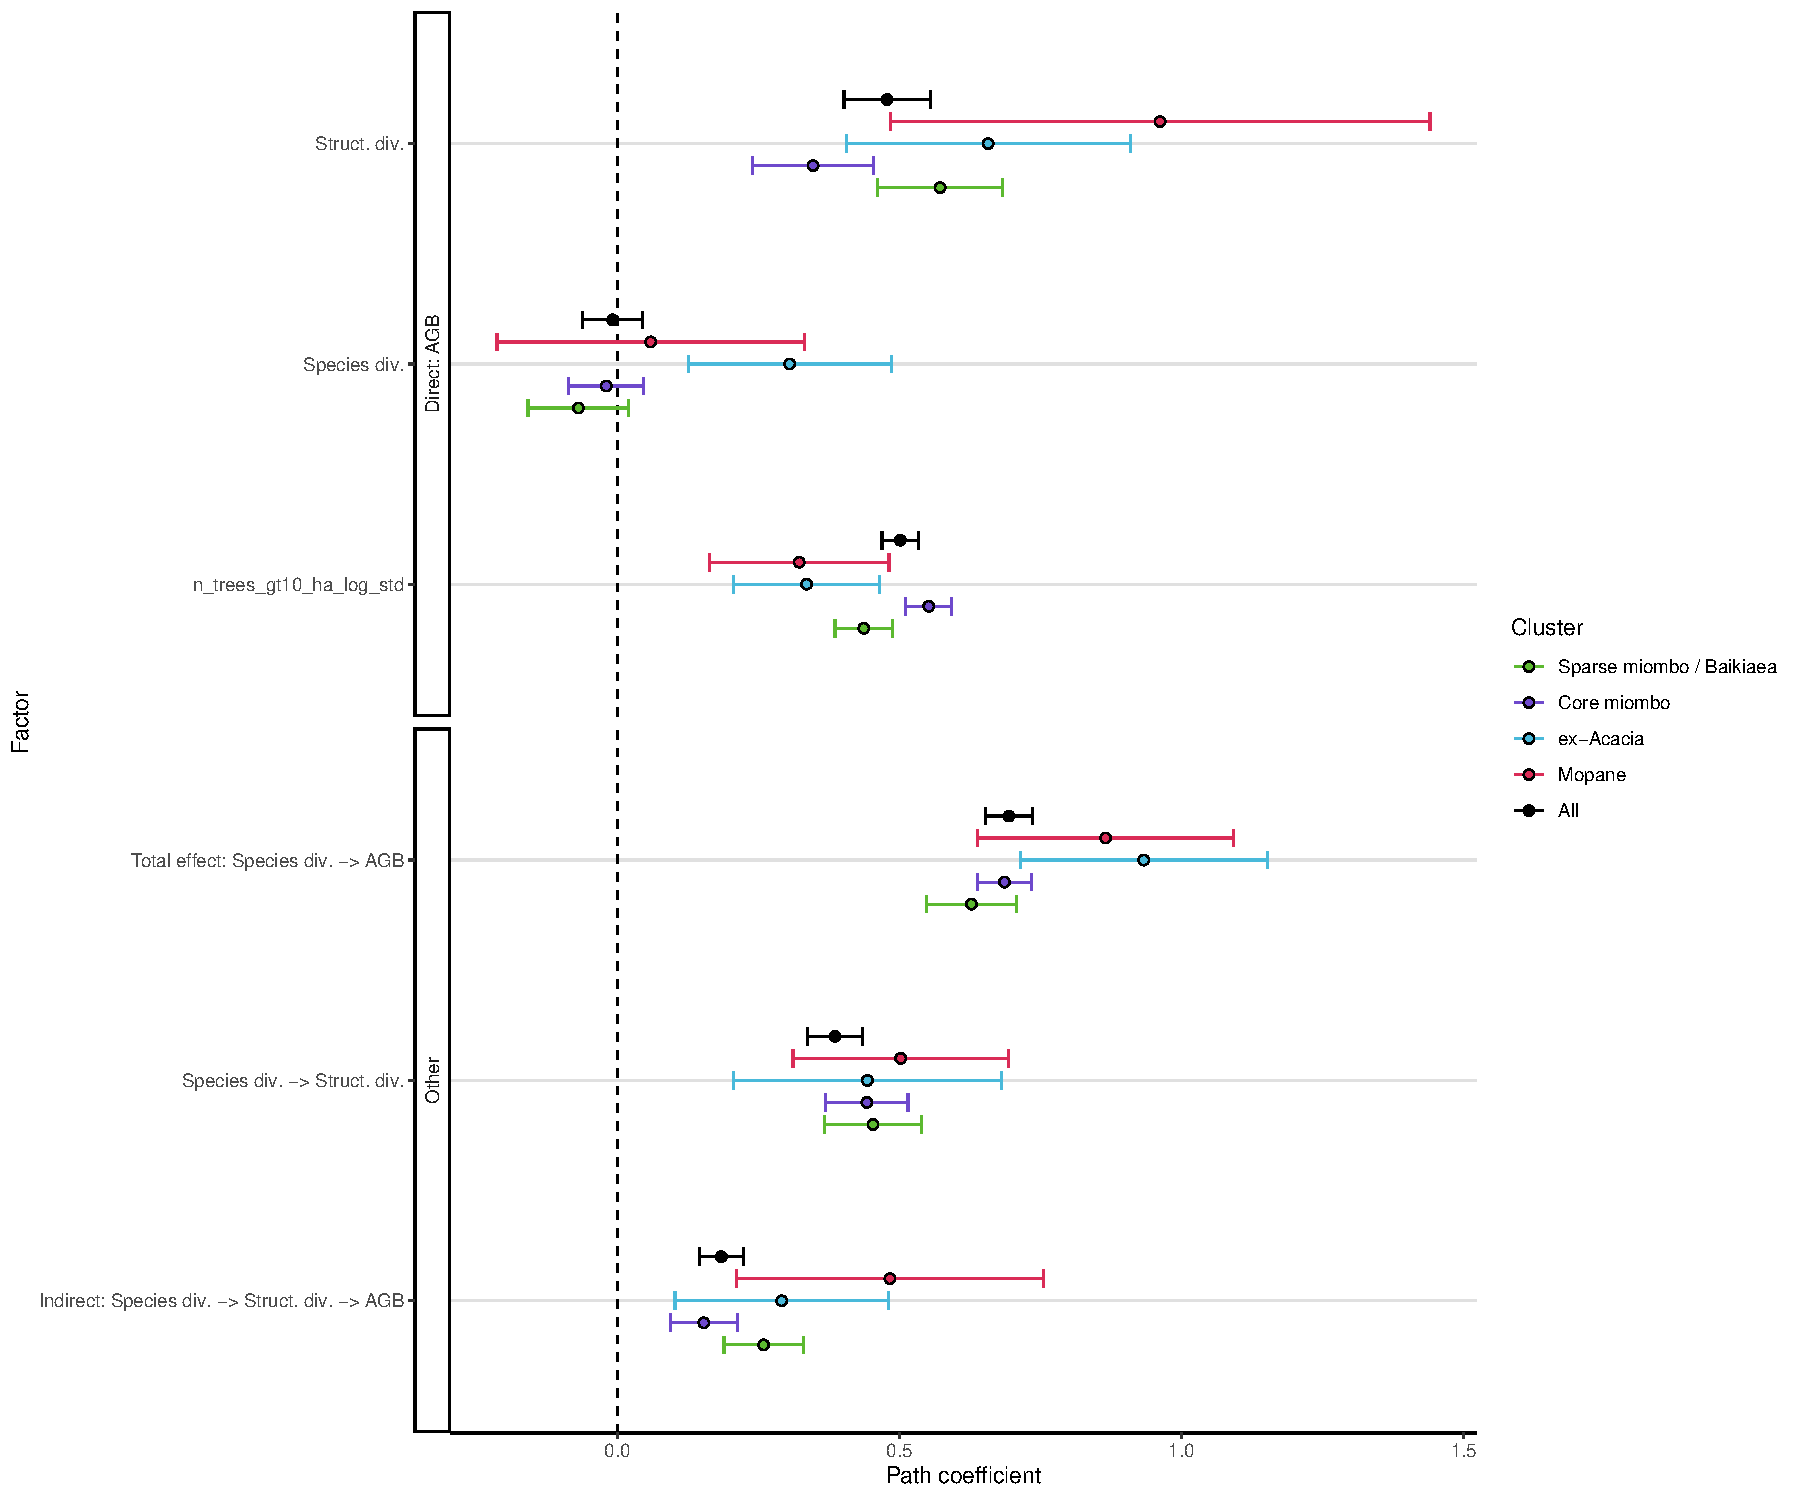
\includegraphics[width=\textwidth]{struc_model_slopes_all}
	\caption{Unstandardised path coefficients for the effects of tree diversity on AGB, mediated by the effect of stand structural diversity. Path coefficients are $\pm$ 1 standard error. Path coefficients where the standard error does not overlap zero are considered to be significant effects.}
	\label{struc_model_slopes_all}
\end{figure}



% Table created by stargazer v.5.2.2 by Marek Hlavac, Harvard University. E-mail: hlavac at fas.harvard.edu
% Date and time: Fri, Jan 17, 2020 - 12:26:16
\begin{table}[!htbp] \centering 
  \caption{} 
  \label{struc_model_fit_clust_stats} 
\begin{tabular}{@{\extracolsep{5pt}} ccccccccc} 
\\[-1.8ex]\hline 
\hline \\[-1.8ex] 
cluster & ntotal & chisq & df & cfi & tli & logl & rmsea & rsquare\_agb \\ 
\hline \\[-1.8ex] 
Marginal miombo & $525$ & $44.750$ & $6$ & $0.966$ & $0.916$ & $$-$3714.000$ & $0.110$ & $0.710$ \\ 
Core miombo & $668$ & $57.210$ & $6$ & $0.962$ & $0.904$ & $$-$4224.000$ & $0.100$ & $0.680$ \\ 
Baikiaea & $47$ & $5.860$ & $6$ & $0.998$ & $0.994$ & $$-$324.600$ & $0.030$ & $0.720$ \\ 
Mopane & $84$ & $9.420$ & $6$ & $0.971$ & $0.927$ & $$-$591.600$ & $0.080$ & $0.450$ \\ 
All & $1324$ & $78.430$ & $6$ & $0.975$ & $0.936$ & $$-$9119.000$ & $0.090$ & $0.690$ \\ 
\hline \\[-1.8ex] 
\end{tabular} 
\end{table} 


\subsubsection{Moderation of Diversity-AGB relationship by stem density}

We repeatedly sub-sampled the plot dataset to build \subn{} datasets of varying mean stem density in order to test how the relationship between species diversity, structural diversity and biomass varied with stem density. Each dataset consisted of approximately \subp{} plots with of plot identity between subsampled datasets. The same SEM specification was used as above (\autoref{struc_mod}) except that stem density was removed.  \autoref{sem_struc_stems_ha} shows a saturating effect of tree species diversity on AGB as stem density increases. There appears to be a minimum stem density threshold at \textapprox{}295 stems ha\textsuperscript{-1} below which there appears to be no effect of tree diversity on biomass. The effect of structural diversity on biomass appears to decrease slightly with increasing stem density, though the relationship is less clear.

\begin{figure}[H]
\centering
	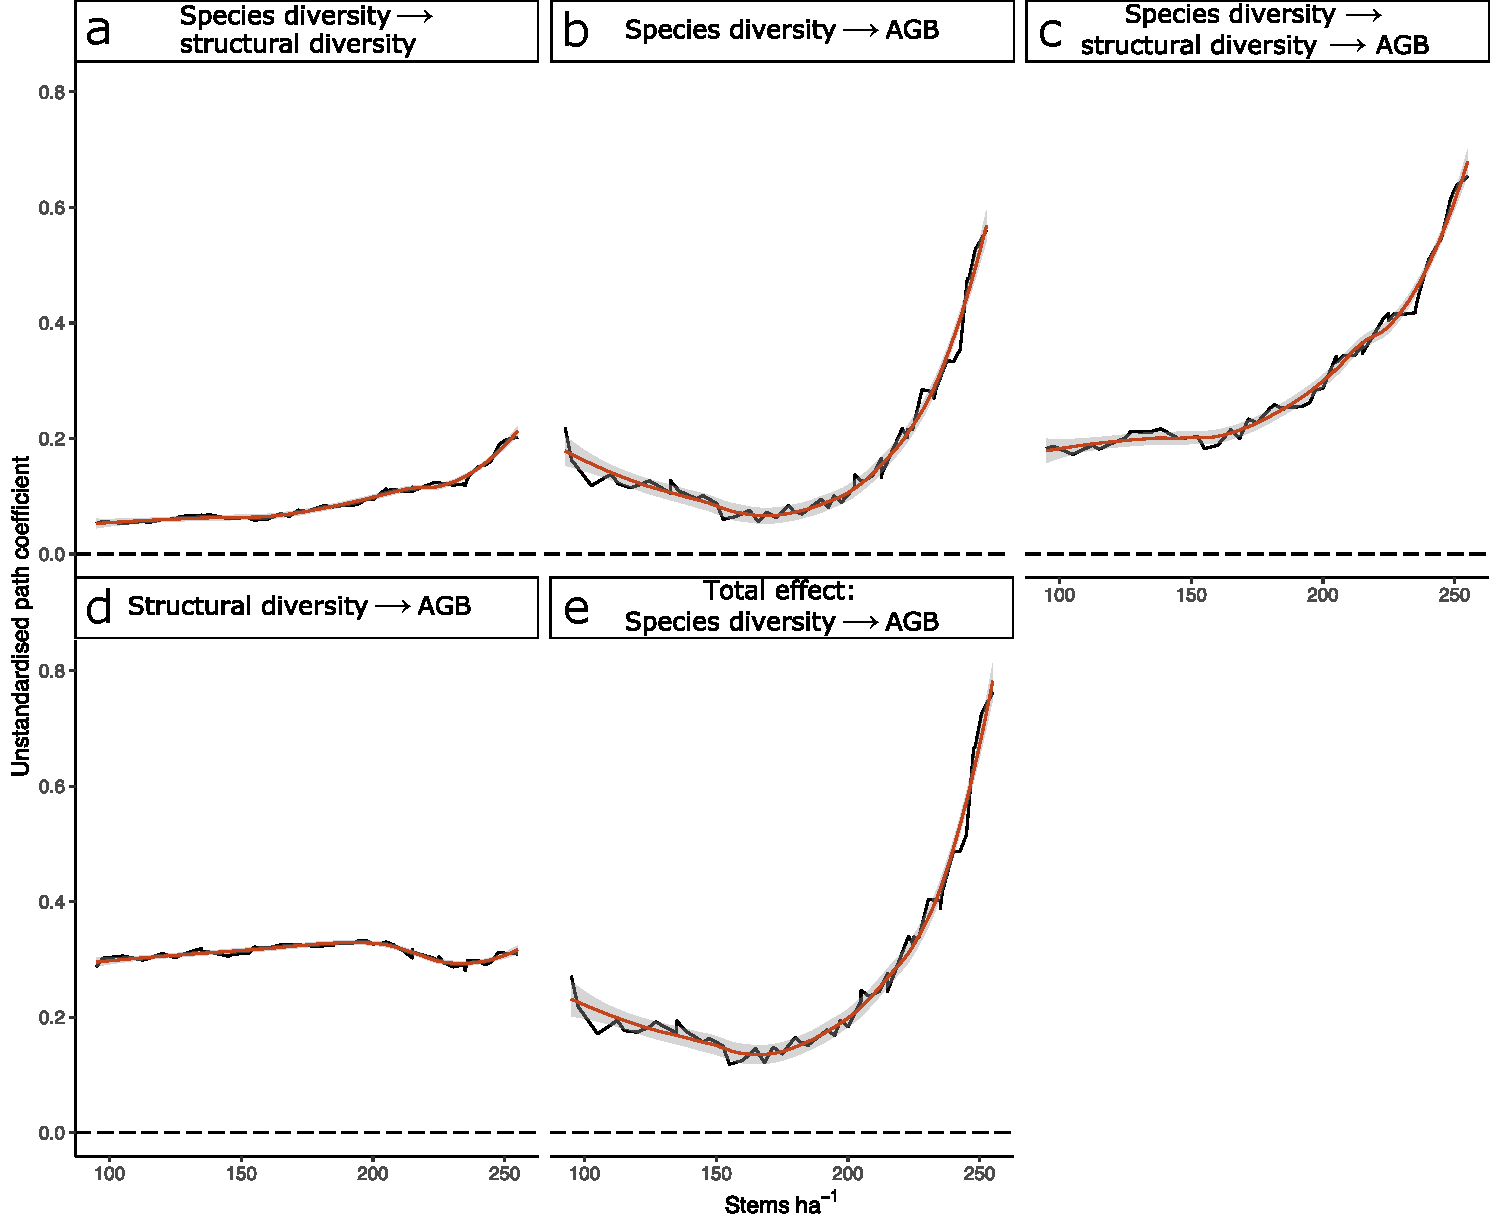
\includegraphics[width=0.8\textwidth]{sem_struc_stems_ha}
	\caption{Line plots showing the variation in path coefficients in the SEM, using datasets with different mean stem density. Smoothed lines are loess curves with standard error shaded bars.}
	\label{sem_struc_stems_ha}
\end{figure}

\subsection{Mediation of environmental covariates via diversity}

A model incorporating the latent variables of moisture availability and soil fertility showed that the effect of diversity on biomass was greater than that of both moisture availability and soil fertility (\autoref{full_mod}). Surprisingly, the direct effects of moisture availability and soil fertility on biomass were negligible, with nearly all of their observed effect on AGB coming from the indirect path via species diversity (moisture: \rgmbd{}, soil: \rgsbd{}) (\autoref{full_model_slopes}). MAP and temperature seasonality had the greatest contributions to the latent variable of moisture availability. Model fit was acceptable: CFI = \fmcfi{}, TLI = \fmtli{}, and RMSEA = \fmrmsea{}. The R\textsuperscript{2} coefficient of determination on AGB was \fmrsq{}.

Moisture availability and soil fertility also had negligible direct effects on stem density, but both had a positive total effect on stem density via species diversity, where species diversity itself had a strong positive effect on stem density (\rgid{}). As species diversity increases, stem density also increases. 

Similar to the model which only considered tree species and structural diversity, the direct effect of species diversity on structural diversity was very weakly positive, while structural diversity itself had a positive effect on AGB (\rghb{}). 

\begin{figure}[H]
\centering
	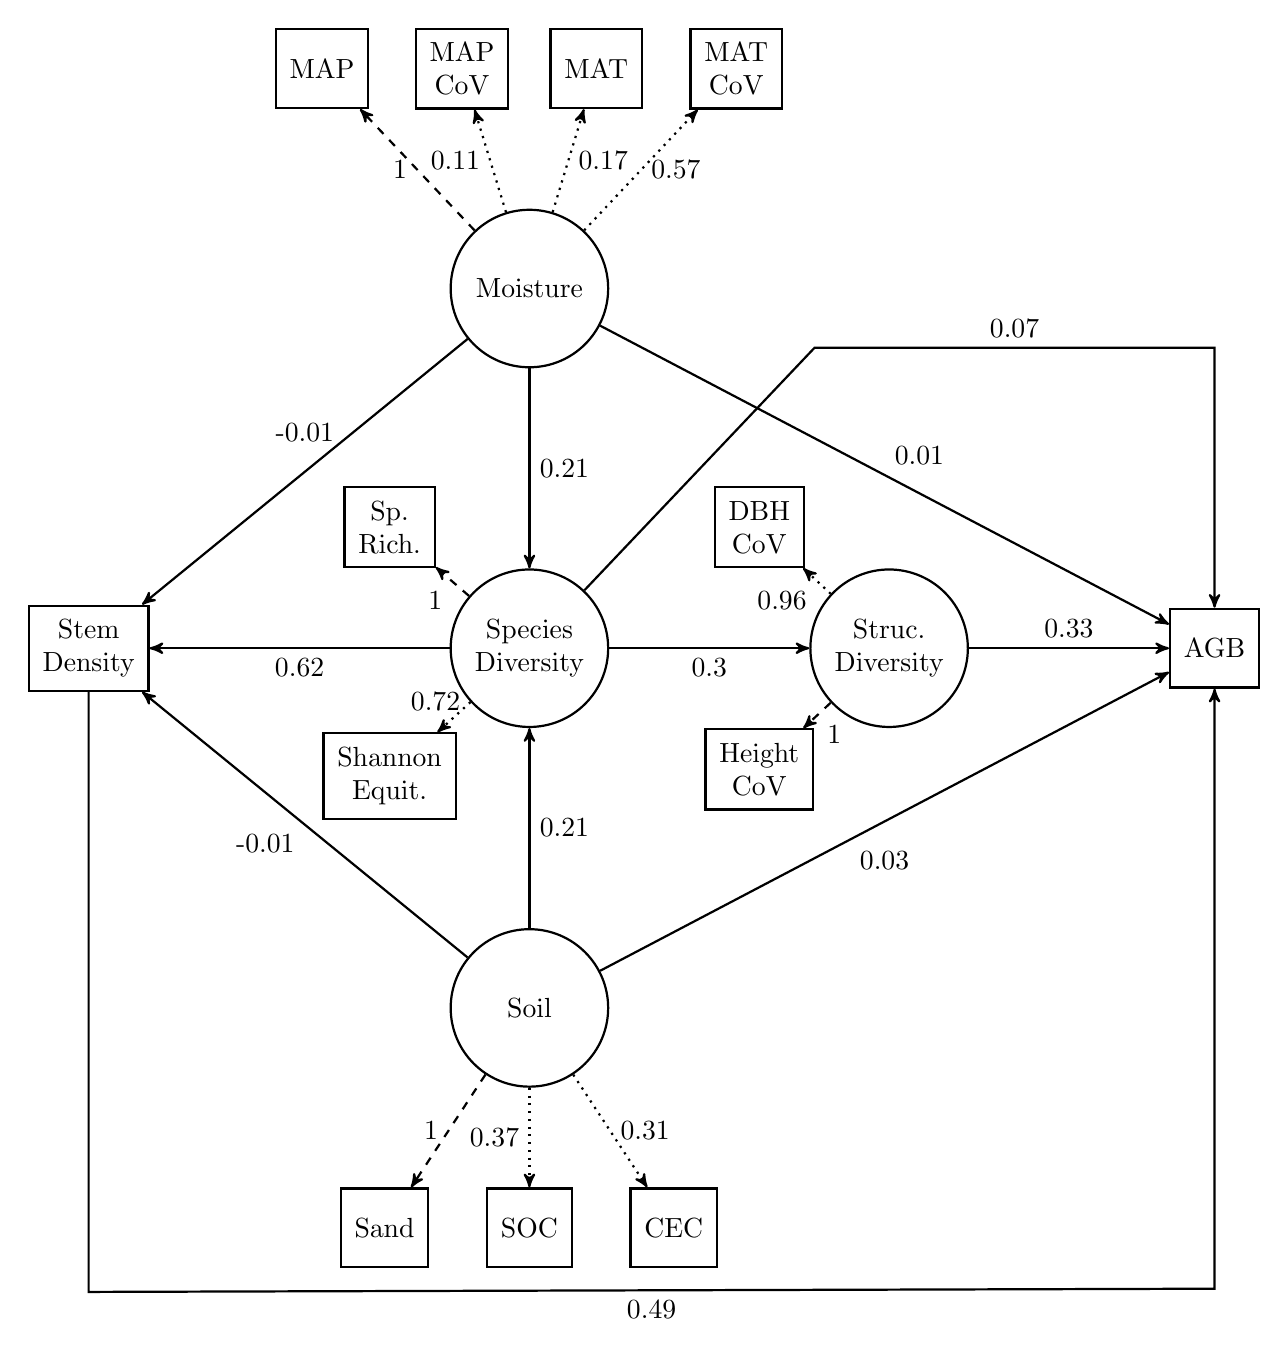
\begin{tikzpicture}[auto,scale=2, 
	observed/.style={rectangle,draw,thick,inner sep=5pt,minimum size=1cm, align=center},
	latent/.style={circle, draw, thick, inner sep=0pt, minimum size=2cm, align=center}, 
	path/.style={->, thick, >=stealth'},
	loading/.style={->, thick, dotted, >=stealth'},
	loadingset/.style={->, thick, dashed, >=stealth'}]

\tikzset{mystyle/.style={->,double=black}}
\node [latent] (m) {Moisture};
\node [latent] (d) [below = 1in of m] {Species\\Diversity}; 
\node [latent] (s) [below = 1in of d] {Soil}; 
\node [latent] (h) [right = 1in of d] {Struc.\\Diversity}; 
\node [observed] (b) [right = 1in of h] {AGB}; 
\node [observed] (i) [left = 1.5in of d] {Stem\\Density};

\coordinate[above= 0.7in of m] (momid);
\node [observed] (mp) [left = 0.8in of momid] {MAP};
\node [observed] (mpc) [left = 0.1in of momid] {MAP\\CoV};
\node [observed] (mt) [right = 0.1in of momid] {MAT};
\node [observed] (mtc) [right = 0.8in of momid] {MAT\\CoV};

\coordinate[below= 0.7in of s] (somid);
\node [observed] (ss) [left = 0.5in of somid] {Sand};
\node [observed] (sc) at (somid) {SOC};
\node [observed] (so) [right = 0.5in of somid] {CEC};

\coordinate[left= 0.3in of d] (domid);
\node [observed] (ds) [above = 0.4in of domid] {Sp.\\Rich.};
\node [observed] (de) [below = 0.42in of domid] {Shannon\\Equit.};

\coordinate[left= 0.25in of h] (homid); 
\node [observed] (hd) [above = 0.4in of homid] {DBH\\CoV};
\node [observed] (hh) [below = 0.4in of homid] {Height\\CoV};


\draw [path] (m) to node {\pcfmd{}} (d);
\draw [path] (s) to node[right] {\pcfsd{}} (d);
\draw [path] (d) to node[below] {\pcfdh{}} (h);
\draw [path] (h) to node {\pcfhb{}} (b);
\draw [path] (m) to node[above=0.1in, pos=0.5] {\pcfmi{}} (i);
\draw [path] (s) to node {\pcfsi{}} (i);
\draw [path] (d) to node {\pcfdi{}} (i);
\draw [path] (m) to node {\pcfmb{}} (b);
\draw [path] (s) to node[below=0.1in, pos=0.5] {\pcfsb{}} (b);

\draw [loadingset] (m) to node[left, pos=0.5] {\pcfmmp{}} (mp);
\draw [loading] (m) to node[left, pos=0.5] {\pcfmmpc{}} (mpc);
\draw [loading] (m) to node[right, pos=0.5] {\pcfmmt{}} (mt);
\draw [loading] (m) to node[right, pos=0.5] {\pcfmmtc{}} (mtc);

\draw [loadingset] (s) to node[left, pos=0.5] {\pcfsss{}} (ss);
\draw [loading] (s) to node[left, pos=0.5] {\pcfssc{}} (sc);
\draw [loading] (s) to node[right, pos=0.5] {\pcfsso{}} (so);

\draw [loadingset] (d) to node {\pcfdds{}} (ds);
\draw [loading] (d) to node[left, pos=0] {\pcfdde{}} (de);

\draw [loading] (h) to node[] {\pcfhhd{}} (hd);
\draw [loadingset] (h) to node {\pcfhhh{}} (hh);

\coordinate[below= 3in of i] (ibleft); 
\coordinate[below= 3in of b] (ibright); 
\draw [path] (i) -- (ibleft) to node[below] {\pcfib{}} (ibright) -- (b);

\coordinate[above= 1.3in of b] (dbright);
\coordinate[left= 2in of dbright] (dbleft);
\draw [path] (d) -- (dbleft) to node[above] {\pcfdb{}} (dbright) -- (b);

\end{tikzpicture}



	\caption{Path diagram with regression coefficients for the SEM incorporating environmental covariates and tree species and structural diversity across all five vegetation type clusters. Latent variables are shown as circles while observed variables are shown as rectangles. Path coefficients are solid arrows pointing from predictor to response. The observed variables which inform the unmeasured latent variables are connected by dotted arrows, observed variables with loading set to one are connected by dashed arrows. Measurement errors of exogenous variables are omitted for clarity.}
	\label{full_mod}
\end{figure}

\begin{figure}[H]
\centering
	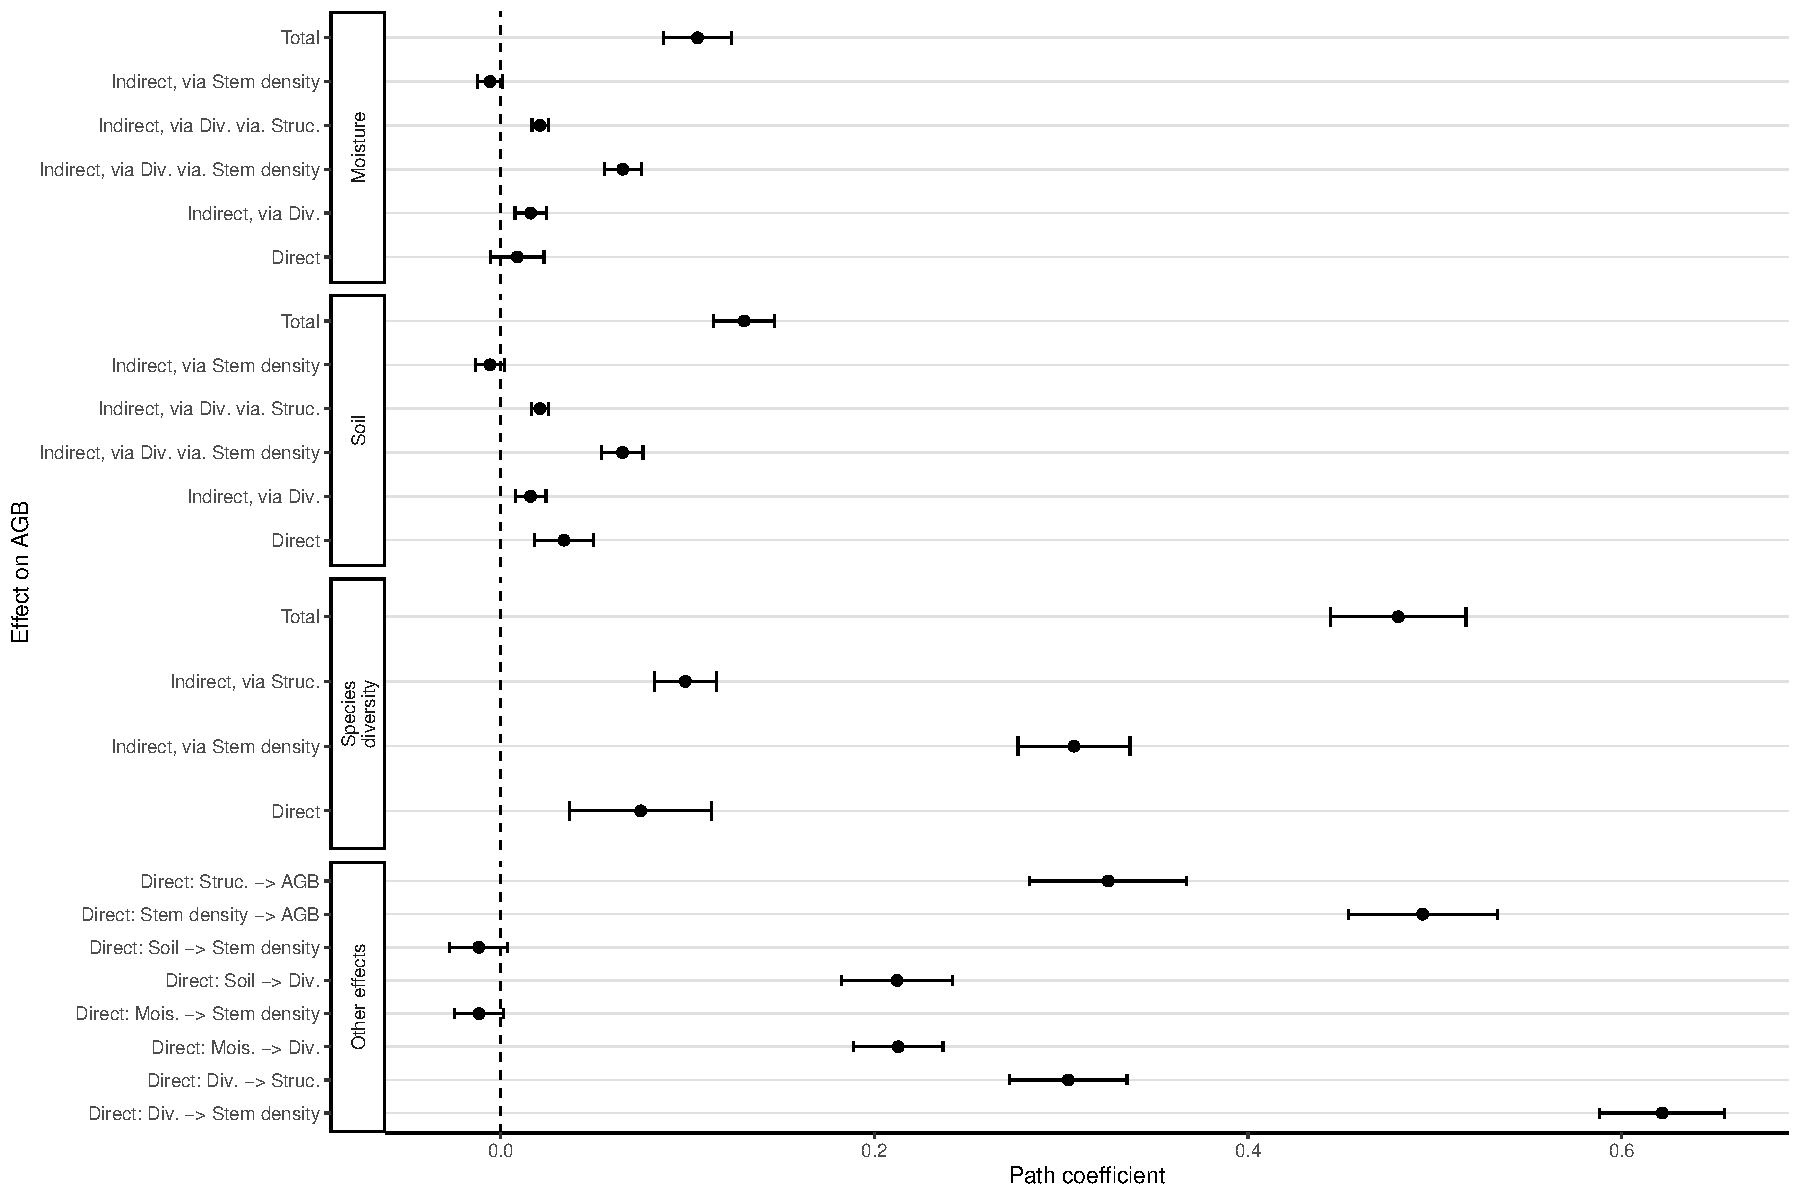
\includegraphics[width=\textwidth]{full_model_slopes}
	\caption{Standardised path coefficients for the interactive effects of abiotic environment and tree diversity on AGB across all plots. Path coefficients are $\pm$ 1 standard error. Path coefficients where the standard error does not overlap zero are considered significant effects.}
	\label{full_model_slopes}
\end{figure}

% 
% Table created by stargazer v.5.2.2 by Marek Hlavac, Harvard University. E-mail: hlavac at fas.harvard.edu
% Date and time: Tue, Oct 29, 2019 - 10:25:05
\begin{table}[!htbp] \centering 
  \caption{} 
  \label{full_model_fit_clust_stats} 
\begin{tabular}{@{\extracolsep{5pt}} ccccccccccc} 
\\[-1.8ex]\hline 
\hline \\[-1.8ex] 
cluster & npar & ntotal & chisq & df & cfi & tli & logl & aic & rmsea & srmr \\ 
\hline \\[-1.8ex] 
C1 & $25$ & $420$ & $1259.430$ & $53$ & $0.460$ & $0.327$ & $$-$6145.100$ & $12340.200$ & $0.230$ & $0.187$ \\ 
C2 & $25$ & $671$ & $1530.040$ & $53$ & $0.445$ & $0.309$ & $$-$8588.900$ & $17227.900$ & $0.200$ & $0.149$ \\ 
C3 & $25$ & $105$ & $516.500$ & $53$ & $0.417$ & $0.274$ & $$-$1055.300$ & $2160.700$ & $0.290$ & $0.216$ \\ 
C4 & $25$ & $46$ & $227.910$ & $53$ & $0.457$ & $0.324$ & $$-$607.600$ & $1265.200$ & $0.270$ & $0.233$ \\ 
C5 & $25$ & $84$ & $489.700$ & $53$ & $0.387$ & $0.237$ & $$-$1097.700$ & $2245.400$ & $0.310$ & $0.328$ \\ 
\hline \\[-1.8ex] 
\end{tabular} 
\end{table} 
 - Excluded, low fit

Vegetation cluster level models could not be reliably fitted for this more complex model specification with environmental covariates, due to sample size issues and because some vegetation clusters were narrow in their climate space. leading to a lack of variance particularly in moisture availability.


\subsection{Moderation effects of moisture availability and soil}

To address the hypothesis (H\textsubscript{2}) that more arid plots and plots with less fertile soil will show a stronger positive effect of tree species richness on above ground woody biomass, we fit separate linear multiple regressions with the latent variables of moisture availability and soil fertility as moderators on the relationship between species diversity and AGB.

Both soil fertility and moisture availability had small positive interaction effects on the strength of the relationship between tree species diversity and biomass (\autoref{int_plots}). The regression coefficient for the interaction effect of tree species diversity and moisture availability was significant (\moderp{}), while the interaction term of tree species diversity and soil fertility was not (\moders{}). As moisture availability increased, the effect of tree species diversity on AGB became stronger. See \autoref{mois_div_int_mod} and \autoref{soil_div_int_mod} for full regression tables.


\begin{figure}[H]
\centering
	\subfloat[]{
	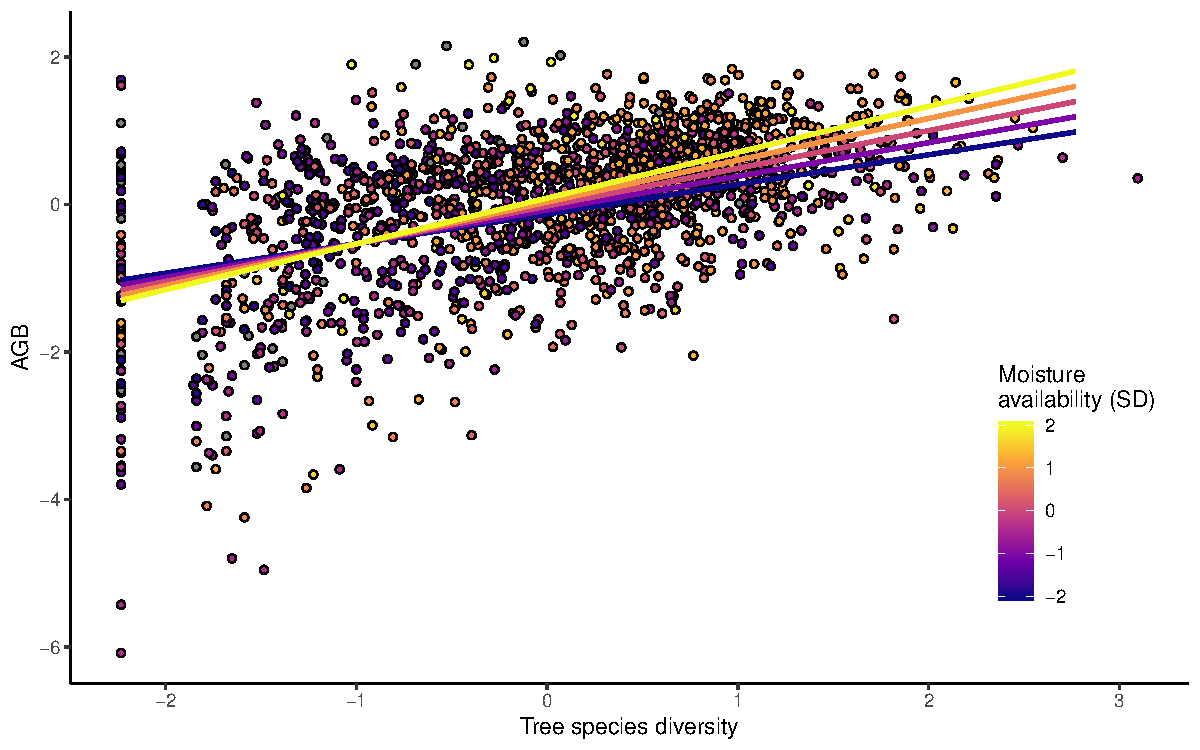
\includegraphics[width=0.48\textwidth]{mois_int}
	}
	\subfloat[]{
	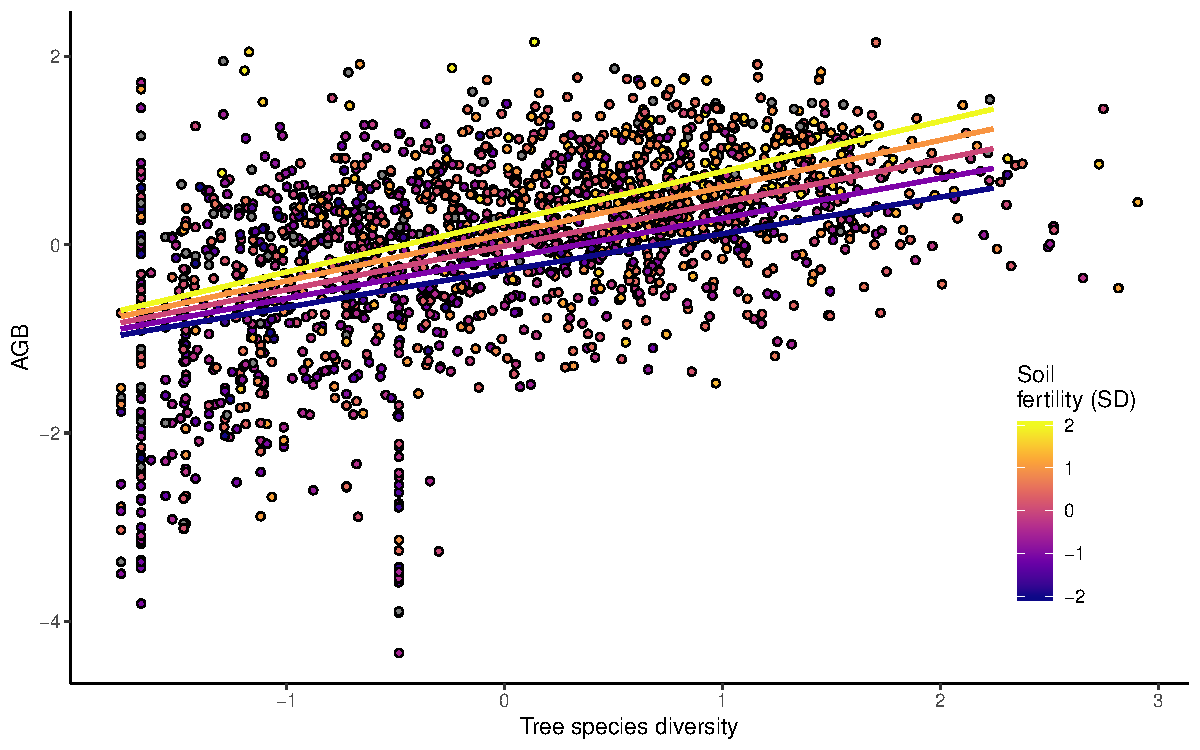
\includegraphics[width=0.48\textwidth]{soil_int}
	}
	\caption{Scatter plots showing variation in the relationship between tree species diversity and AGB with moisture availability (a) and soil fertility (b). All variables are standardised and centred to a mean of zero and a standard deviation of 1. Lines of best fit are drawn for standard deviations of moisture availability and soil fertility between -2 and +2. Moisture availability, tree species diversity and soil fertility are latent variables comprised of the same observed variable loadings.}
	\label{int_plots}
\end{figure}

\section{Discussion}

%1. Plots with a higher tree species diversity will maintain higher above-ground woody biomass stocks.
%2. More arid plots and plots with less fertile soil will show a stronger positive effect of tree species richness on above-ground woody biomass.
%3. There will be a positive effect of precipitation and soil fertility on AGB and that part of this positive effect will exist as a mediating effect through species diversity.
%4. Structural characteristics of the woodland will interact with species diversity to provide an indirect path of influence between species composition and biomass stocks.
%5. The observed effect of diversity on AGB will increase in strength as stem density increases owing to an increased importance of niche complementarity as competition increases.

In this study, we assessed the importance of [a] tree species richness, [b] tree structural diversity, [c] moisture availability and soil fertility, [d] stem density and their interactions on aboveground woody biomass (AGB) across southern African woodlands, using a plot network of \nplots{}. Using latent variables and Structural Equation Modelling (SEM), we found support for a general relationship between tree species diversity and AGB (H\textsubscript{1}), and an indirect relationship between tree species diversity and AGB via structural diversity (H\textsubscript{4}) and via stem density (H\textsubscript{5}). Tree diversity and stem density accounted for 46\% of the variation in AGB across the region, while models for certain vegetation types showed even greater explanatory power. The strongest effect on AGB was that of stem density, which itself was highly dependent on species diversity. Interestingly, when tree species diversity, structural diversity and stem density were controlled for, we found little evidence of a direct effect of resource availability, in the form of moisture availability and soil fertility, on AGB (H\textsubscript{3}). In separate multiple regressions however, we did find weak indirect moderation effects of both soil fertility and moisture availability on the strength of the relationship between species diversity and AGB (H\textsubscript{2}). We found that vegetation composition in the form of discrete vegetation type clusters affected the relationship between species diversity and AGB, with true Miombo woodland representing an outlier in our models (vegetation type cluster C2).

\todo{Why is Cluster 2 different?}

\todo{C3 had the strongest effect of species div on AGB}


\subsection{Effect of tree species diversity on AGB}

The latent variable of tree species diversity had a strong positive effect on woody above-ground biomass (AGB) in the environment+diversity SEM model (\autoref{full_mod}). Within the savanna woodlands of southern Africa we therefore find support for our hypothesis (H\textsubscript{1}), that higher tree species richness causes higher woody AGB. This finding is in agreement with many other studies across different ecosystems and biomes, showing that there is a generalisable positive association between species richness and ecosystem functionality \citep{Liang2016, Cardinale2009}. 

Most of the total species diversity effect was through the indirect effect via stem density. This suggests that within southern African woodlands a higher species diversity allows for a greater density of tree stems and this leads to an increase in total AGB. While reverse causation is plausible, with increased stem density causing higher species richness through an increased probability of encountering new species, we accounted for this variation via the extrapolation of species richness according to stem density (sampling effort), meaning that stem density should have little causal effect on species diversity in our models. This suggests that the observed direction of causation in our model is real. We cannot decompose the relative effects of tree species richness and abundance evenness in our model, but previous studies have shown that both richness and evenness have similar importance in their effects on ecosystem function \citep{Valery2009, Zhang2012}. We suggest that an increase in tree species diversity through species richness and evenness produces an assemblage of species which can occupy a greater proportion of the total woodland canopy volume with leaf area, utilising more of the available light resulting in greater total AGB at the plot level. This is supported by the moderately strong positive effect of tree species diversity on AGB via structural diversity.

% The question of whether lots of small stems or a few large stems maximises AGB has yet to be solved \citep{}.

While we did not explicitly measure net primary production (NPP) in this study, other studies have shown a strong positive correlation between woody AGB and NPP in woodland and forest ecosystems \citep{Chisholm2013, Prado-Junior2016}. This suggests that as has been found in many other woodland/forest ecosystems, woody biomass and woody productivity in southern African woodlands can be maximised by increasing species diversity. 

\subsection{Structural diversity as a mechanism for the BEFR}

We found evidence that species diversity led to an increase in AGB via tree structural diversity, we can therefore accept our hypothesis (H\textsubscript{4}). A higher tree species diversity allows for a greater diversity of tree functional forms within a plot and this may act as a mechanism of niche complementarity, with a highly diverse canopy being able to take advantage of a greater proportion of the available light. Variation in structural diversity may be a joint result of disturbance history and tree species diversity, with highly disturbed plots generally having a less structurally diverse canopy \citep{LaRue2019}. In forests, where the tree canopy is effectively closed, as the stand matures a more diverse canopy emerges via competition and tree mortality events which open canopy gaps \citep{Muscolo2014}. In highly disturbed woodland plots, we suggest that disturbance history may be an important unmeasured abiotic factor which may account for a high proportion of the variation in AGB and in tree species diversity. In highly disturbed forests, maturity in the sense of classical forest succession is never reached, and a simple open canopy is maintained. Unfortunately we did not have access to a dataset of high enough spatial and temporal resolution to adequately quantify the effects of disturbance history. 

\subsection{Effects of moisture availability and soil fertility}

Surprisingly, moisture availability and soil fertility had only small effects on AGB compared to that of tree species diversity. We expected that higher moisture availability and soil fertility would lead to higher AGB under the assumption that higher resource availability would allow for greater resource partitioning between individual trees \citep{} and a greater stem density per unit area \citep{}.

Previous studies in tropical forests have shown that moisture availability increases AGB both directly and indirectly via increasing tree species diversity and via increasing stand structural diversity \citep{Ali2019a, Ali2019b, Poorter2017}. In this study, while we observed the indirect effects on species diversity, we saw no evidence for a direct effect on AGB. Compared to moist tropical forests, climatic water availability is more of a limiting factor to tree growth in southern African woodlands, which are frequently droughted. It is possible that the range of observed moisture availability in this study (\textapprox{}460-1700 mm y\textsuperscript{-1}) may not have been able to capture variation in AGB. We deliberately exlcuded plots with very low stem density as they are not considered woodlands, but grassy savannas. It may be that by excluding the bottom end of this stem density continuum we prevented a relationship being observed between moisture and AGB/stem density. Additionally, due to the high levels of adaptation of tree species to drought conditions in southern Africa, at the large scale we conducted our experiment turnover in species composition may have prevented a direct relationship being observed between resource availability and AGB.

In southern African woodlands moisture availability is closely linked with the intensity of disturbance from seasonal fires. The growth of C4 grasses in wetter woodlands leads to more intense seasonal fires which limit tree growth \citep{Charles-Dominique2018}, and may also limit species diversity \citep{Linder2014}. It is possible therefore that the effect of moisture availabiliy is confounded in it effect on AGB with the unmeasured variable of intensity of disturbance by fire. The direct effect of moisture availability on stem density may also be confounded in this way.

In a separate set of linear multiple regressions, we found a weak positive interaction effect of moisture availability on the relationship between tree species diversity and AGB. As moisture availability increased, the relationship between tree species diversity and AGB became stronger. This is in contrast to \citet{Ratcliffe2017} who found that in European forests, a decrease in water availability due to drought led to a stronger effect of tree species diversity on AGB. They attributed this to an increase in selection effects which allowed dominance of stress tolerant species which were more likely to occur in high diversity assemblages. \todo{Why were our results different?} 

\subsection{Vegetation type cluster specific responses}

\todo{I have no idea what to write here just yet}

\subsection{Stem density effects}

We found a non linear saturating effect of stem density on the relationship between tree species diversity and AGB (\autoref{sem_struc_stems_ha}). The effect of tree species diversity on AGB peaked at \textapprox{}700 stems ha\textsuperscript{-1}. At low stem densities competition between trees may not occur, meaning that the niche complementarity provided by an increase in tree species richness might not make any difference to plot level AGB.

It is possible that at very high stem density there are other factors which become more important than tree species diversity in affecting AGB. For example, very high stem density plots in our dataset often had tree species commonly found in thicket vegetation, which is highly structured through disturbance by fire. There may also be an effect whereby the high stem density plots have many small stems, meaning that AGB cannot be high. An abundance of small stems may prevent the growth of large trees which hold the majority of the AGB in a plot. The peak in species diversity effect may occur at a given stem density due to a balance point between tree species diversity effects and the offsetting effects of stem crowding which preclude high biomass large trees.

\todo{Maybe at very low stem density, no niche complementarity}

\todo{Decreasing effect of struct. on AGB with stem density}

% Seidel 2019: Large trees tend to possess a greater structural complexity than small trees, not due to their size per se, but due to more complex architecture.

% At very high biomass, tree species diversity is low because it is associated with intense competition for light leading to dominance of usually a single species (Huston 1997, Oindo and Skidmore 2002).


% \subsection{Future work}

% We hope that this study prompts further investigation of the relationship between woody productuivity and species richness and composition in southern African woodlands. While AGB is correlated with NPP,...

\subsection{Conclusion}

\bibliography{/Users/johngodlee/google_drive/bib/lib.bib}

\newpage{}
\appendix{}

\section*{Appendix 1 - Data cleaning process}

\begin{figure}[H]
\centering
	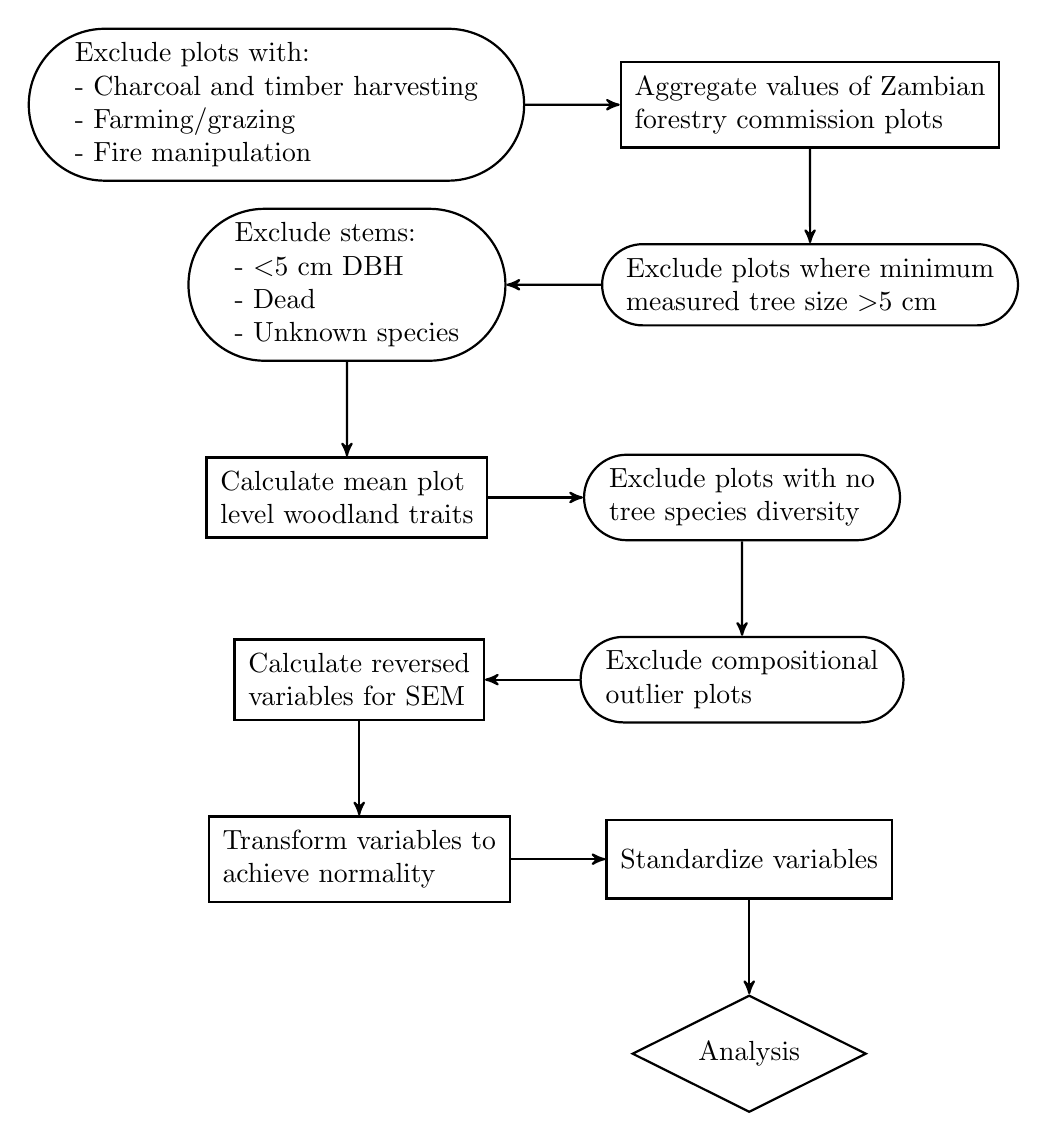
\begin{tikzpicture}[auto,scale=2, 
	round/.style={rounded rectangle,draw,thick,inner sep=5pt,minimum size=1cm, align=left},
	box/.style={rectangle,draw,thick,inner sep=5pt,minimum size=1cm, align=left},
	diam/.style={diamond,draw,thick,inner sep=5pt,minimum size=1cm, align=left, aspect=2},
	path/.style={->, thick, >=stealth'}]

\tikzset{mystyle/.style={->,double=black}}
\node  [round] (a)                    {Exclude plots with:\\- Charcoal and timber  harvesting\\- Farming/grazing\\- Fire manipulation};
\node  [box] (b) [right = 1.2cm of a] {Aggregate values of Zambian\\forestry commission plots};
\node  [round] (c) [below = 1.2cm of b] {Exclude plots where minimum\\measured tree size \textgreater{}5 cm};
\node  [round] (d) [left = 1.2cm of c] {Exclude stems:\\- \textless{}5 cm DBH\\- Dead\\- Unknown species};
\node  [box] (e) [below = 1.2cm of d] {Calculate mean plot\\level woodland traits};
\node  [round] (f) [right = 1.2cm of e] {Exclude plots with no\\tree species diversity};
\node  [round] (g) [below = 1.2cm of f] {Exclude compositional\\outlier plots};
\node  [box] (h) [left = 1.2cm of g] {Calculate reversed\\variables for SEM};
\node  [box] (i) [below = 1.2cm of h] {Transform variables to\\achieve normality};
\node  [box] (j) [right = 1.2cm of i] {Standardize variables};
\node  [diam] (k) [below = 1.2cm of j] {Analysis};
\draw [path] (a) -> (b);
\draw [path] (b) -> (c);
\draw [path] (c) -> (d);
\draw [path] (d) -> (e);
\draw [path] (e) -> (f);
\draw [path] (f) -> (g);
\draw [path] (g) -> (h);
\draw [path] (h) -> (i);
\draw [path] (i) -> (j);
\draw [path] (j) -> (k);

\end{tikzpicture}

	\caption{Flow diagram of the data filtering and cleaning process prior to analysis. Rounded boxes indicate filtering events while regular boxes indicate calculation events.}
	\label{data_clean_flow}
\end{figure}

\section*{Appendix 2 - Table of correlation fit statistics}


% Table created by stargazer v.5.2.2 by Marek Hlavac, Harvard University. E-mail: hlavac at fas.harvard.edu
% Date and time: Wed, Jun 24, 2020 - 13:33:02
\begin{table}[!htbp] \centering 
  \caption{} 
  \label{corr_ci_tab} 
\begin{tabular}{@{\extracolsep{5pt}} ccccccc} 
\\[-1.8ex]\hline 
\hline \\[-1.8ex] 
x\_var & y\_var & raw.r & raw.lower & raw.upper & n & p \\ 
\hline \\[-1.8ex] 
Sand \% & Org. C (ppt) & $$-$0.620$ & $$-$0.650$ & $$-$0.580$ & $1235$ & p \textless 0.01 \\ 
Sand \% & CEC & $$-$0.510$ & $$-$0.550$ & $$-$0.470$ & $1235$ & p \textless 0.01 \\ 
Sand \% & MAP & $$-$0.500$ & $$-$0.540$ & $$-$0.460$ & $1235$ & p \textless 0.01 \\ 
Sand \% & PS & $0.350$ & $0.300$ & $0.400$ & $1235$ & p \textless 0.01 \\ 
Sand \% & MAT & $0.340$ & $0.280$ & $0.380$ & $1235$ & p \textless 0.01 \\ 
Sand \% & TS & $0.380$ & $0.330$ & $0.430$ & $1235$ & p \textless 0.01 \\ 
Sand \% & Sp. rich. & $$-$0.330$ & $$-$0.370$ & $$-$0.280$ & $1235$ & p \textless 0.01 \\ 
Sand \% & Shannon equit. & $0.250$ & $0.190$ & $0.300$ & $1235$ & p \textless 0.01 \\ 
Sand \% & Tree height CV & $$-$0.250$ & $$-$0.300$ & $$-$0.190$ & $981$ & p \textless 0.01 \\ 
Sand \% & DBH CV & $$-$0.170$ & $$-$0.230$ & $$-$0.120$ & $1233$ & p \textless 0.01 \\ 
Sand \% & Stems ha & $$-$0.100$ & $$-$0.160$ & $$-$0.050$ & $1235$ & p \textless 0.01 \\ 
Sand \% & AGB & $$-$0.270$ & $$-$0.320$ & $$-$0.220$ & $1235$ & p \textless 0.01 \\ 
Org. C (ppt) & CEC & $0.460$ & $0.410$ & $0.500$ & $1235$ & p \textless 0.01 \\ 
Org. C (ppt) & MAP & $0.440$ & $0.390$ & $0.480$ & $1235$ & p \textless 0.01 \\ 
Org. C (ppt) & PS & $$-$0.410$ & $$-$0.450$ & $$-$0.360$ & $1235$ & p \textless 0.01 \\ 
Org. C (ppt) & MAT & $$-$0.280$ & $$-$0.330$ & $$-$0.230$ & $1235$ & p \textless 0.01 \\ 
Org. C (ppt) & TS & $$-$0.280$ & $$-$0.330$ & $$-$0.230$ & $1235$ & p \textless 0.01 \\ 
Org. C (ppt) & Sp. rich. & $0.150$ & $0.090$ & $0.200$ & $1235$ & p \textless 0.01 \\ 
Org. C (ppt) & Shannon equit. & $$-$0.160$ & $$-$0.220$ & $$-$0.110$ & $1235$ & p \textless 0.01 \\ 
Org. C (ppt) & Tree height CV & $0.180$ & $0.120$ & $0.240$ & $981$ & p \textless 0.01 \\ 
Org. C (ppt) & DBH CV & $0.140$ & $0.080$ & $0.190$ & $1233$ & p \textless 0.01 \\ 
Org. C (ppt) & Stems ha & $0.090$ & $0.030$ & $0.140$ & $1235$ & p \textless 0.01 \\ 
Org. C (ppt) & AGB & $0.270$ & $0.220$ & $0.320$ & $1235$ & p \textless 0.01 \\ 
CEC & MAP & $$-$0.070$ & $$-$0.130$ & $$-$0.020$ & $1235$ & p \textless 0.01 \\ 
CEC & PS & $$-$0.590$ & $$-$0.630$ & $$-$0.550$ & $1235$ & p \textless 0.01 \\ 
CEC & MAT & $0.170$ & $0.120$ & $0.220$ & $1235$ & p \textless 0.01 \\ 
CEC & TS & $0.070$ & $0.010$ & $0.120$ & $1235$ & p \textless 0.05 \\ 
CEC & Sp. rich. & $$-$0.100$ & $$-$0.160$ & $$-$0.050$ & $1235$ & p \textless 0.01 \\ 
CEC & Shannon equit. & $$-$0.120$ & $$-$0.180$ & $$-$0.070$ & $1235$ & p \textless 0.01 \\ 
CEC & Tree height CV & $0.090$ & $0.020$ & $0.150$ & $981$ & p \textless 0.01 \\ 
CEC & DBH CV & $0.130$ & $0.080$ & $0.190$ & $1233$ & p \textless 0.01 \\ 
CEC & Stems ha & $$-$0.090$ & $$-$0.140$ & $$-$0.030$ & $1235$ & p \textless 0.01 \\ 
CEC & AGB & $0.080$ & $0.030$ & $0.140$ & $1235$ & p \textless 0.01 \\ 
MAP & PS & $$-$0.070$ & $$-$0.130$ & $$-$0.020$ & $1235$ & p \textless 0.05 \\ 
MAP & MAT & $$-$0.200$ & $$-$0.260$ & $$-$0.150$ & $1235$ & p \textless 0.01 \\ 
MAP & TS & $$-$0.770$ & $$-$0.790$ & $$-$0.740$ & $1235$ & p \textless 0.01 \\ 
MAP & Sp. rich. & $0.400$ & $0.350$ & $0.450$ & $1235$ & p \textless 0.01 \\ 
MAP & Shannon equit. & $$-$0.130$ & $$-$0.180$ & $$-$0.070$ & $1235$ & p \textless 0.01 \\ 
MAP & Tree height CV & $0.250$ & $0.190$ & $0.310$ & $981$ & p \textless 0.01 \\ 
MAP & DBH CV & $0.120$ & $0.060$ & $0.170$ & $1233$ & p \textless 0.01 \\ 
MAP & Stems ha & $0.070$ & $0.010$ & $0.120$ & $1235$ & p \textless 0.05 \\ 
MAP & AGB & $0.230$ & $0.180$ & $0.280$ & $1235$ & p \textless 0.01 \\ 
precip\_seas\_std & MAT & $0$ & $$-$0.050$ & $0.060$ & $1235$ & p = 0.95 \\ 
precip\_seas\_std & TS & $0.140$ & $0.080$ & $0.190$ & $1235$ & p \textless 0.01 \\ 
precip\_seas\_std & Sp. rich. & $0.130$ & $0.070$ & $0.180$ & $1235$ & p \textless 0.01 \\ 
precip\_seas\_std & Shannon equit. & $0.070$ & $0.010$ & $0.130$ & $1235$ & p \textless 0.05 \\ 
precip\_seas\_std & Tree height CV & $$-$0.060$ & $$-$0.120$ & $0.010$ & $981$ & p = 0.07 \\ 
precip\_seas\_std & DBH CV & $$-$0.100$ & $$-$0.150$ & $$-$0.040$ & $1233$ & p \textless 0.01 \\ 
precip\_seas\_std & Stems ha & $$-$0.030$ & $$-$0.080$ & $0.030$ & $1235$ & p = 0.33 \\ 
precip\_seas\_std & AGB & $$-$0.190$ & $$-$0.240$ & $$-$0.130$ & $1235$ & p \textless 0.01 \\ 
MAT & TS & $0.060$ & $0$ & $0.120$ & $1235$ & p \textless 0.05 \\ 
MAT & Sp. rich. & $$-$0.170$ & $$-$0.220$ & $$-$0.120$ & $1235$ & p \textless 0.01 \\ 
MAT & Shannon equit. & $0$ & $$-$0.060$ & $0.060$ & $1235$ & p = 0.98 \\ 
MAT & Tree height CV & $$-$0.040$ & $$-$0.100$ & $0.020$ & $981$ & p = 0.2 \\ 
MAT & DBH CV & $0.060$ & $0.010$ & $0.120$ & $1233$ & p \textless 0.05 \\ 
MAT & Stems ha & $$-$0.150$ & $$-$0.210$ & $$-$0.100$ & $1235$ & p \textless 0.01 \\ 
MAT & AGB & $$-$0.090$ & $$-$0.150$ & $$-$0.040$ & $1235$ & p \textless 0.01 \\ 
TS & Sp. rich. & $$-$0.440$ & $$-$0.480$ & $$-$0.390$ & $1235$ & p \textless 0.01 \\ 
TS & Shannon equit. & $0.200$ & $0.150$ & $0.250$ & $1235$ & p \textless 0.01 \\ 
TS & Tree height CV & $$-$0.210$ & $$-$0.270$ & $$-$0.150$ & $981$ & p \textless 0.01 \\ 
TS & DBH CV & $$-$0.090$ & $$-$0.150$ & $$-$0.040$ & $1233$ & p \textless 0.01 \\ 
TS & Stems ha & $$-$0.050$ & $$-$0.110$ & $0.010$ & $1235$ & p = 0.08 \\ 
TS & AGB & $$-$0.180$ & $$-$0.230$ & $$-$0.120$ & $1235$ & p \textless 0.01 \\ 
Sp. rich. & Shannon equit. & $$-$0.580$ & $$-$0.620$ & $$-$0.540$ & $1235$ & p \textless 0.01 \\ 
Sp. rich. & Tree height CV & $0.300$ & $0.250$ & $0.360$ & $981$ & p \textless 0.01 \\ 
Sp. rich. & DBH CV & $0.300$ & $0.250$ & $0.350$ & $1233$ & p \textless 0.01 \\ 
Sp. rich. & Stems ha & $0.240$ & $0.190$ & $0.300$ & $1235$ & p \textless 0.01 \\ 
Sp. rich. & AGB & $0.310$ & $0.260$ & $0.360$ & $1235$ & p \textless 0.01 \\ 
Shannon equit. & Tree height CV & $$-$0.120$ & $$-$0.190$ & $$-$0.060$ & $981$ & p \textless 0.01 \\ 
Shannon equit. & DBH CV & $$-$0.200$ & $$-$0.250$ & $$-$0.140$ & $1233$ & p \textless 0.01 \\ 
Shannon equit. & Stems ha & $$-$0.410$ & $$-$0.460$ & $$-$0.360$ & $1235$ & p \textless 0.01 \\ 
Shannon equit. & AGB & $$-$0.350$ & $$-$0.400$ & $$-$0.300$ & $1235$ & p \textless 0.01 \\ 
Tree height CV & DBH CV & $0.470$ & $0.420$ & $0.520$ & $981$ & p \textless 0.01 \\ 
Tree height CV & Stems ha & $0.010$ & $$-$0.060$ & $0.070$ & $981$ & p = 0.86 \\ 
Tree height CV & AGB & $0.240$ & $0.180$ & $0.290$ & $981$ & p \textless 0.01 \\ 
DBH CV & Stems ha & $0.110$ & $0.060$ & $0.170$ & $1233$ & p \textless 0.01 \\ 
DBH CV & AGB & $0.430$ & $0.390$ & $0.480$ & $1233$ & p \textless 0.01 \\ 
Stems ha & AGB & $0.590$ & $0.550$ & $0.620$ & $1235$ & p \textless 0.01 \\ 
\hline \\[-1.8ex] 
\end{tabular} 
\end{table} 


\section*{Appendix 3 - Frequency distribution of observed variables}

\begin{figure}[H]
\centering
	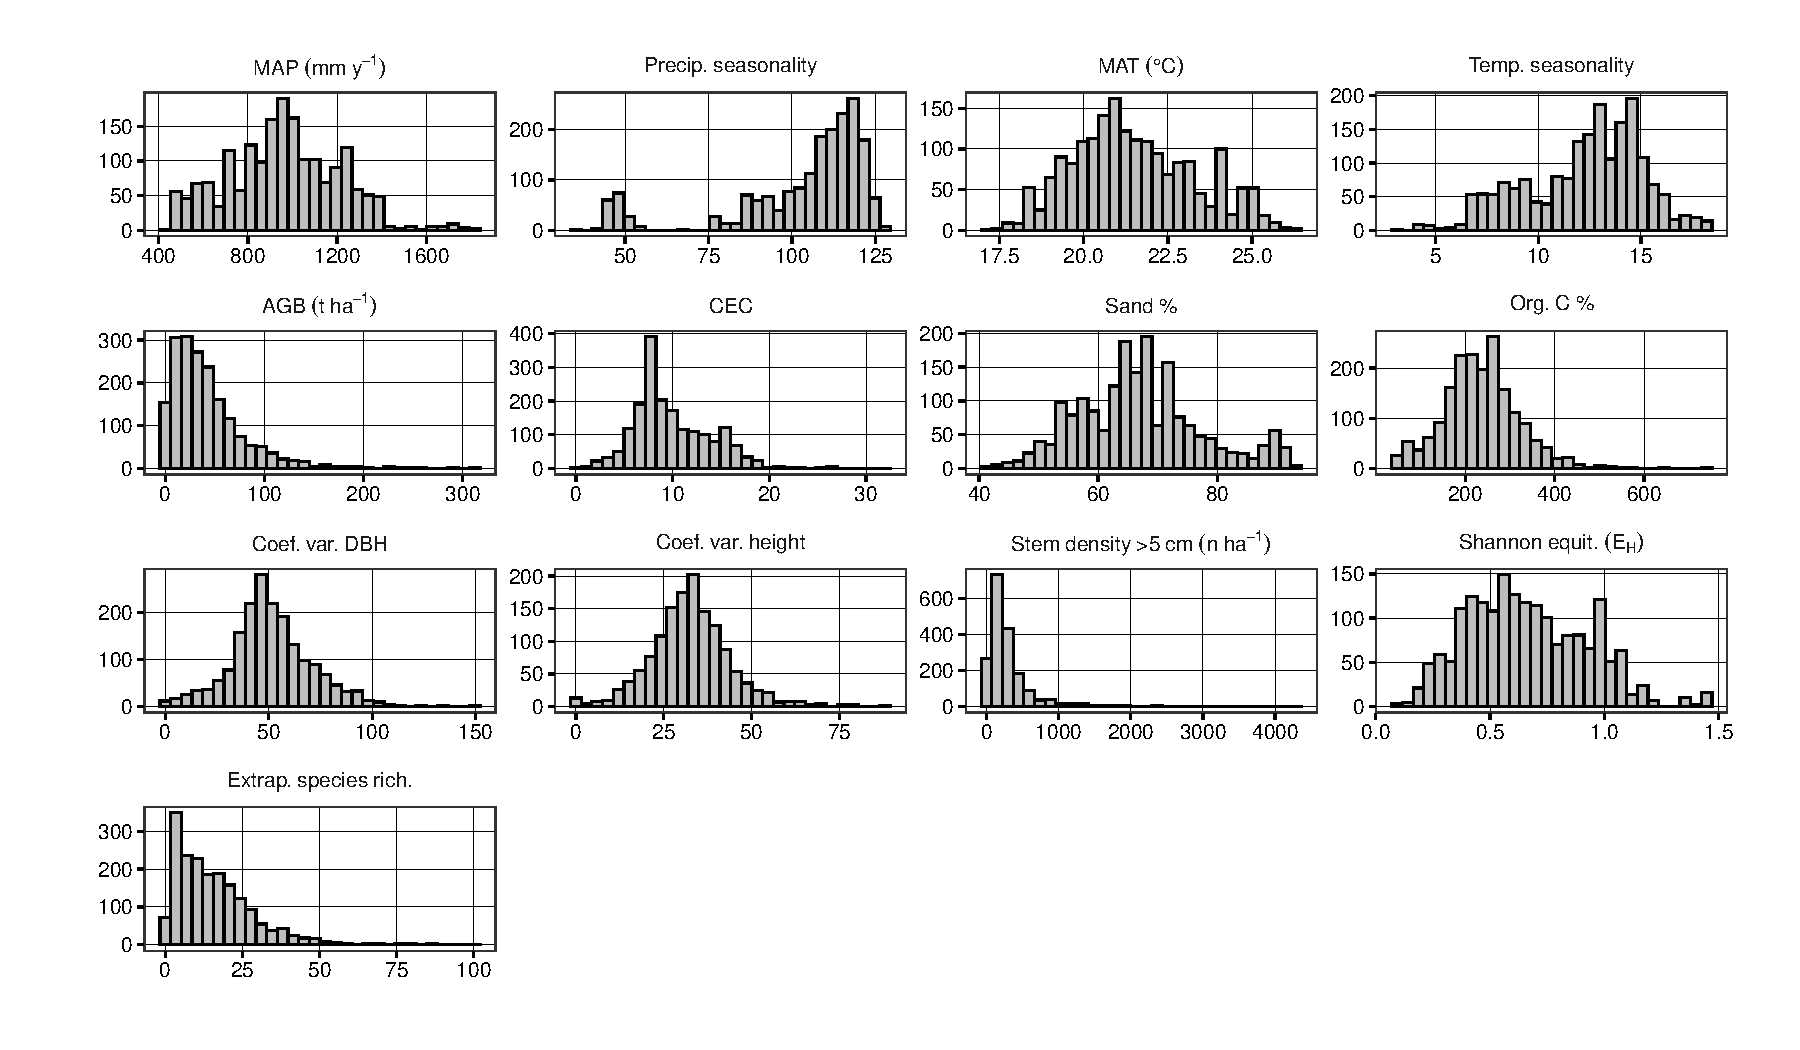
\includegraphics[width=\textwidth]{histogram_raw_obs}
	\caption{Histograms of raw untransformed observed variables used in final analyses.}
	\label{histogram_raw_obs}
\end{figure}

\begin{figure}[H]
\centering
	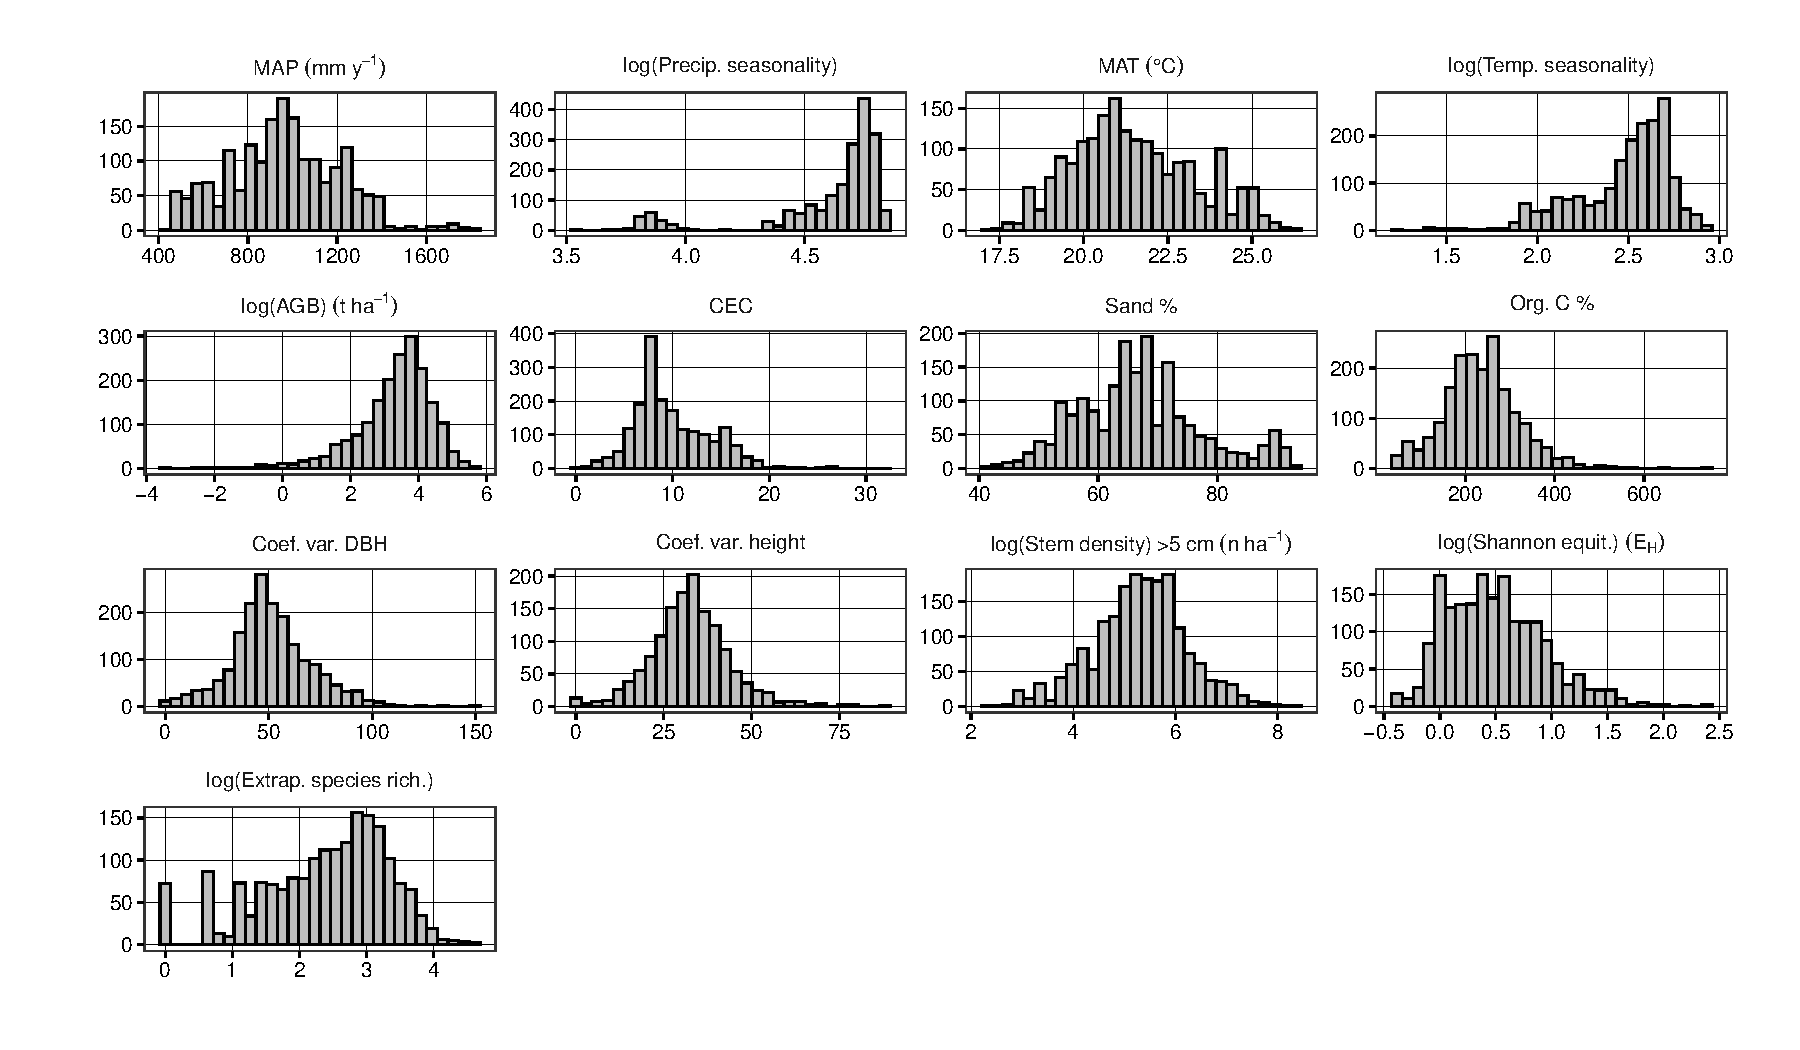
\includegraphics[width=\textwidth]{histogram_trans_obs}
	\caption{Histograms of observed variables transformed to achieve a normal frequency distribution.}
	\label{histogram_trans_obs}
\end{figure}

\section*{Appendix 4 - Regression tables for moderation by environmental variables}


% Table created by stargazer v.5.2.2 by Marek Hlavac, Harvard University. E-mail: hlavac at fas.harvard.edu
% Date and time: Tue, Dec 17, 2019 - 16:41:22
\begin{table}[!htbp] \centering 
  \caption{} 
  \label{mois_div_int_mod} 
\begin{tabular}{@{\extracolsep{5pt}}lc} 
\\[-1.8ex]\hline 
\hline \\[-1.8ex] 
 & \multicolumn{1}{c}{\textit{Dependent variable:}} \\ 
\cline{2-2} 
\\[-1.8ex] & agb\_ha\_log\_std\_std \\ 
\hline \\[-1.8ex] 
 n\_species\_raref\_log\_std\_std & 0.465$^{***}$ \\ 
  & (0.022) \\ 
  & \\ 
 total\_precip\_std\_std & 0.095$^{***}$ \\ 
  & (0.022) \\ 
  & \\ 
 n\_species\_raref\_log\_std\_std:total\_precip\_std\_std & 0.004 \\ 
  & (0.021) \\ 
  & \\ 
 Constant & $-$0.001 \\ 
  & (0.022) \\ 
  & \\ 
\hline \\[-1.8ex] 
Observations & 1,769 \\ 
R$^{2}$ & 0.256 \\ 
Adjusted R$^{2}$ & 0.255 \\ 
Residual Std. Error & 0.863 (df = 1765) \\ 
F Statistic & 202.726$^{***}$ (df = 3; 1765) \\ 
\hline 
\hline \\[-1.8ex] 
\multicolumn{2}{r}{$^{*}$p$<$0.1; $^{**}$p$<$0.05; $^{***}$p$<$0.01} \\ 
\end{tabular} 
\end{table} 



% Table created by stargazer v.5.2.2 by Marek Hlavac, Harvard University. E-mail: hlavac at fas.harvard.edu
% Date and time: Wed, Nov 27, 2019 - 10:09:08
\begin{table}[!htbp] \centering 
  \caption{} 
  \label{soil_div_int_mod} 
\begin{tabular}{@{\extracolsep{5pt}}lc} 
\\[-1.8ex]\hline 
\hline \\[-1.8ex] 
 & \multicolumn{1}{c}{\textit{Dependent variable:}} \\ 
\cline{2-2} 
\\[-1.8ex] & bchave\_std \\ 
\hline \\[-1.8ex] 
 sp\_rich\_raref\_log\_std\_std & 0.480$^{***}$ \\ 
  & (0.022) \\ 
  & \\ 
 ocdens\_std\_std & 0.120$^{***}$ \\ 
  & (0.022) \\ 
  & \\ 
 sp\_rich\_raref\_log\_std\_std:ocdens\_std\_std & 0.036$^{*}$ \\ 
  & (0.021) \\ 
  & \\ 
 Constant & $-$0.014 \\ 
  & (0.022) \\ 
  & \\ 
\hline \\[-1.8ex] 
Observations & 1,766 \\ 
R$^{2}$ & 0.284 \\ 
Adjusted R$^{2}$ & 0.283 \\ 
Residual Std. Error & 0.847 (df = 1762) \\ 
F Statistic & 233.151$^{***}$ (df = 3; 1762) \\ 
\hline 
\hline \\[-1.8ex] 
\multicolumn{2}{r}{$^{*}$p$<$0.1; $^{**}$p$<$0.05; $^{***}$p$<$0.01} \\ 
\end{tabular} 
\end{table} 




\end{document}


% https://jslefche.github.io/sem_book/coefficients.html

